\chapter{Splicing signatures of progressive tau pathology in AD mouse model}\label{ch: transcriptional_global_differences}

\section{Introduction}
There is increasing evidence that transcriptional dysregulation and aberrant splicing plays a role in the development and pathogenesis of AD (described in \cref{intro:AD_alteredsplicing}). Recent transcriptome profiling studies have identified changes in splicing and transcript expression in both human AD post-mortem brain tissue and AD mouse models (reviewed in \cref{tab: AS_ADHuman_studies} and \cref{tab: AS_ADMouse_studies}, respectively). To date, however, these studies have relied on short-read RNA-Sequencing approaches, which cannot reliably detect specific isoforms (as discussed in \cref{rnaseq_intro}).  In contrast, we have illustrated the power of long-read sequencing to identify full-length transcripts and improve our annotations of alternatively spliced isoforms in the cortex of the rTg4510 mouse model of AD tauopathy (\cref{ch: whole_transcriptome}). 

While long-read sequencing approaches are currently considered to be only semi-quantitative, recent studies have delivered promising strategies for transcript-based analysis by using a hybrid approach\cite{Tseng2021}: the alignment of short-read RNA-seq data to improved transcriptome annotations derived from long-read data. This has enabled the identification of differentially expressed isoforms and the analysis of differential isoform usage between experimental groups\cite{Tseng2021}. 

Following on from the results presented in \textbf{Chapter 4}, this chapter aimed to exploit the cortical long-read sequencing datasets generated from rTg4510 transgenic (TG) and wild-type (WT) control mice to identify transcriptional and splicing changes associated with progressive tau pathology. The objectives of this chapter were: 
\begin{enumerate}
	\item To assess global variation in splicing patterns between rTg4510 TG and WT mice
	\item To perform differential gene expression analysis and validate changes in gene expression associated with tau pathology from previous RNA-Seq studies 
	\item To perform differential transcript expression analysis to identify changes in transcript expression associated with tau pathology   
	\item To perform differential transcript usage analysis to identify genes with significant alterations in isoform proportions between rTg4510 transgenic and control mice 
	\item To integrate differential splicing changes with epigenetic data (DNA methylation) available from the same samples.
\end{enumerate} 

\newpage
\section{Methods}

\subsection{Datasets}
All analyses presented in this chapter follow on from \cref{ch: whole_transcriptome} and use the same Iso-Seq long-read datasets generated from 12 female mice (WT = 6, rTg4510 TG = 6, aged 2 and 8 months, \cref{tab:whole_phenotype}). Briefly, RNA was prepared for Iso-Seq library preparation and SMRT sequencing on the PacBio Sequel (\cref{ch4_methods: isoseq_library}), followed by QC and data processing (\cref{ch4_methods: isoseq_data}). Reads from individual samples were processed separately with \textit{IsoSeq3} and merged for transcript collapse with \textit{Cupcake}, genome alignment with \textit{Minimap2}(v2.17) and re-annotation with \textit{SQANTI3} with no splice junction filtering from short-read RNA-Seq data. ISM transcripts with only the 3' fragment matching reference transcript (3'ISM) were considered technical artefacts resulting from 5'degradation and thus removed.  

\subsection{Quantification of human MAPT transgene expression} 
The presence of human- and mouse-specific \textit{Mapt/MAPT} sequences was determined in FL transcripts as a QC check of sample identity. Species-specific \textit{Mapt/MAPT} sequence, located in a 2kb region present in the 3'UTR, was identified after using BLAT\cite{Kent2002} to compare human and mouse MAPT/Mapt sequence for divergent transcript sequences \cite{Castanho2020}).  

\subsection{Characterisation of Alternative Splicing Events} 
Alternative splicing events were examined using a range of packages and custom scripts (as described and implemented in \cref{ch4: transcriptome_annotation}), to assess whether there was a difference in splicing patterns associated with progressive tau pathology in the rTg4510 mouse model. 

\subsection{Gene and Isoform Quantification}
Gene and isoform expression were estimated using two approaches (described in \cref{sec: gene_isoform_quant_explained}). Briefly these were: i) the alignment of short-read RNA-Seq reads to the Iso-Seq-defined transcriptome (hybrid approach) using \textit{Kallisto}\cite{Bray2016} (v0.46.0), and ii) the use of normalised Iso-Seq FL read counts as proxy for expression. FL read counts for each sample were taken from the \textit{read\_stat.txt} file generated using the \textit{collapse\_isoforms\_by\_sam.py} script (\textit{Cupcake}), using the sequencing run ID as identifier. 

\subsection{Differential expression analysis}
Differential expression analysis was performed with \textit{tappAS} (fully described in \cref{ch3_tappas_explained}). Briefly, \textit{tappAS} filters out lowly-expressed isoforms, normalises read counts using TMM approach and performs differential expression analysis using \textit{maSigPro}\cite{Conesa2006,Nueda2014,Conesa2017} to elucidate effects for both genotype and age with the following adapted model\cite{Conesa2006}: 

\vspace{1cm}
\begin{myequation}[h]
Let \textit{I} denote the genotype groups (wild-type - WT, transgenic - TG) and \textit{J} as the age (2 and 8 months) for each particular group, and assuming that gene or transcript expression in measured in replicated samples (\textit{R}).  
\begin{align}
	y_{ijr} =  \:&\beta_{0} + \beta_{1}D_{ijr} \nonumber
	\\ &+ \delta_{0}T_{ijr} + \delta_{1}T_{ijr}D_{ijr}   \nonumber
\end{align}
where
\begin{conditions*}
	y_{ijr} & normalised expression value for each gene or transcript in the situation \textit{ijr} (genotype group \textit{i} at age \textit{j} of replicate \textit{r}) \\
	D  &  dummy binary variable to distinguish between the genotype groups, whereby 0 refers to reference group (WT) and 1 refers to experimental group (TG) \\
	T  &  age at 2 8 months described using a polynomial model with a degree of 1 \\
	\beta_{0}, \delta_{0}, \gamma_{0}, \lambda _{0} & regression coefficients for reference group (WT) relating to the age \\ 
	\beta_{1}, \delta_{1}, \gamma_{1}, \lambda _{1} & regression coefficients for the difference between the experimental group (TG) and reference group (WT) at each age  
\end{conditions*}
therefore, if:
\begin{conditions*}
	FDR(\beta_{1}) < 0.05 & significant expression difference between WT and TG at 2 months \\ 
	FDR(\delta_{0}) < 0.05 & significant expression difference in WT across 2 and 8 months \\
\end{conditions*}
\captionsetup{width=1\textwidth}
\caption[Linear regression model to determine differential gene and transcript expression]%
{\textbf{Linear regression model to determine differential gene and transcript expression}. The model, adapted from \textit{MaSigPro} and implemented as part of \textit{tappAS}, describes gene or transcript expression between two groups (WT - wild-type, TG - transgenic) at four different time points (age in months). FDR - False discovery rate}    
\end{myequation}

\begin{figure}[!htp]
	\centering
	\includegraphics[page=2,trim={0 5cm 0 4cm},scale = 0.45]{Figures/Tg4510_diff_figures.pdf}
	\captionsetup{width=0.95\textwidth}
	\caption[Different conditions modelled for rTg4510 genotype and age effects]%
	{\textbf{Different conditions modelled for rTg4510 genotype and age effects.} Statistical models generated to dissect genotype and age effects with \textit{maSigPro} using \textbf{Equation 5.1} for 2 experimental groups (WT - wild-type/Control, TG - Transgenic/Case) across two time points/age (T1, T2). 
	\\\\
	The regression coefficients from \textbf{Equation 5.1} - $\beta_{1}$, $\delta_{0}$, $\delta_{1}$ - refer to the different variables modelled, the significance of which can be used to infer whether there is a genotype, age or interaction effect. The significance is symbolised by the tick and cross, which refers to adjusted p-value (FDR) < 0.05 and > 0.05 respectively. A significance of  $\beta_{1}$ denotes to a statistically significant difference between WT and TG at T1 (Genotype effect),$\delta_{0}$ to a difference in WT over time (Age effect), and $\delta_{1}$ to a difference between WT and TG across age (Interaction effect).}   
	\label{fig:dea_model}
\end{figure}

Under this model, a differentially expressed gene or transcript between WT and TG mice across age was defined with a statistically significant coefficient (adjusted p-value < 0.05) and a regression model with R\textsuperscript{2} > 0.5  (\cref{fig:dea_model}) .


\clearpage 
\section{Results}
\subsection{PacBio Iso-Seq run performance and sequencing metrics}
No significant difference in sequencing yield was identified between WT and TG mice (n = 12 animals, two-tailed unpaired t-test, t(10) = -0.636, P = 0.539, \cref{fig:rTg4510_sequencing_metrics}\textbf{A}), and no significant correlation was observed between run yield and RIN across samples (n = 12 animals, Pearson's correlation, t = -0.98, df = 10, P = 0.350, \cref{fig:rTg4510_sequencing_metrics}\textbf{B}). No difference was observed in the number of reads (\cref{fig:rTg4510_sequencing_metrics}\textbf{C}) and transcripts generated between WT and TG (n = 12, two-tailed unpaired t-test, t = -0.005, df = 10, P = 0.996, \cref{fig:rTg4510_sequencing_metrics}\textbf{E}) or by age (n = 12, t = -1.58, df = 10, P = 0.15). Notably, a similar read profile was attained for all the samples except the first two samples, which were sequenced using an older chemistry and had a relatively lower throughput. Nonetheless, all the samples were successfully sequenced with optimal runs, as indicated by the high throughput and the similar number of FL, FLNC and Poly-A FLNC reads recovered. ERCC alignment and annotations similarly revealed no difference in number of ERCC molecules detected between WT and TG (mean number of ERCC: WT = 32.4 (35\%), TG = 32.2 (35.22\%)). 

\begin{figure}[htp]
	\begin{center}
		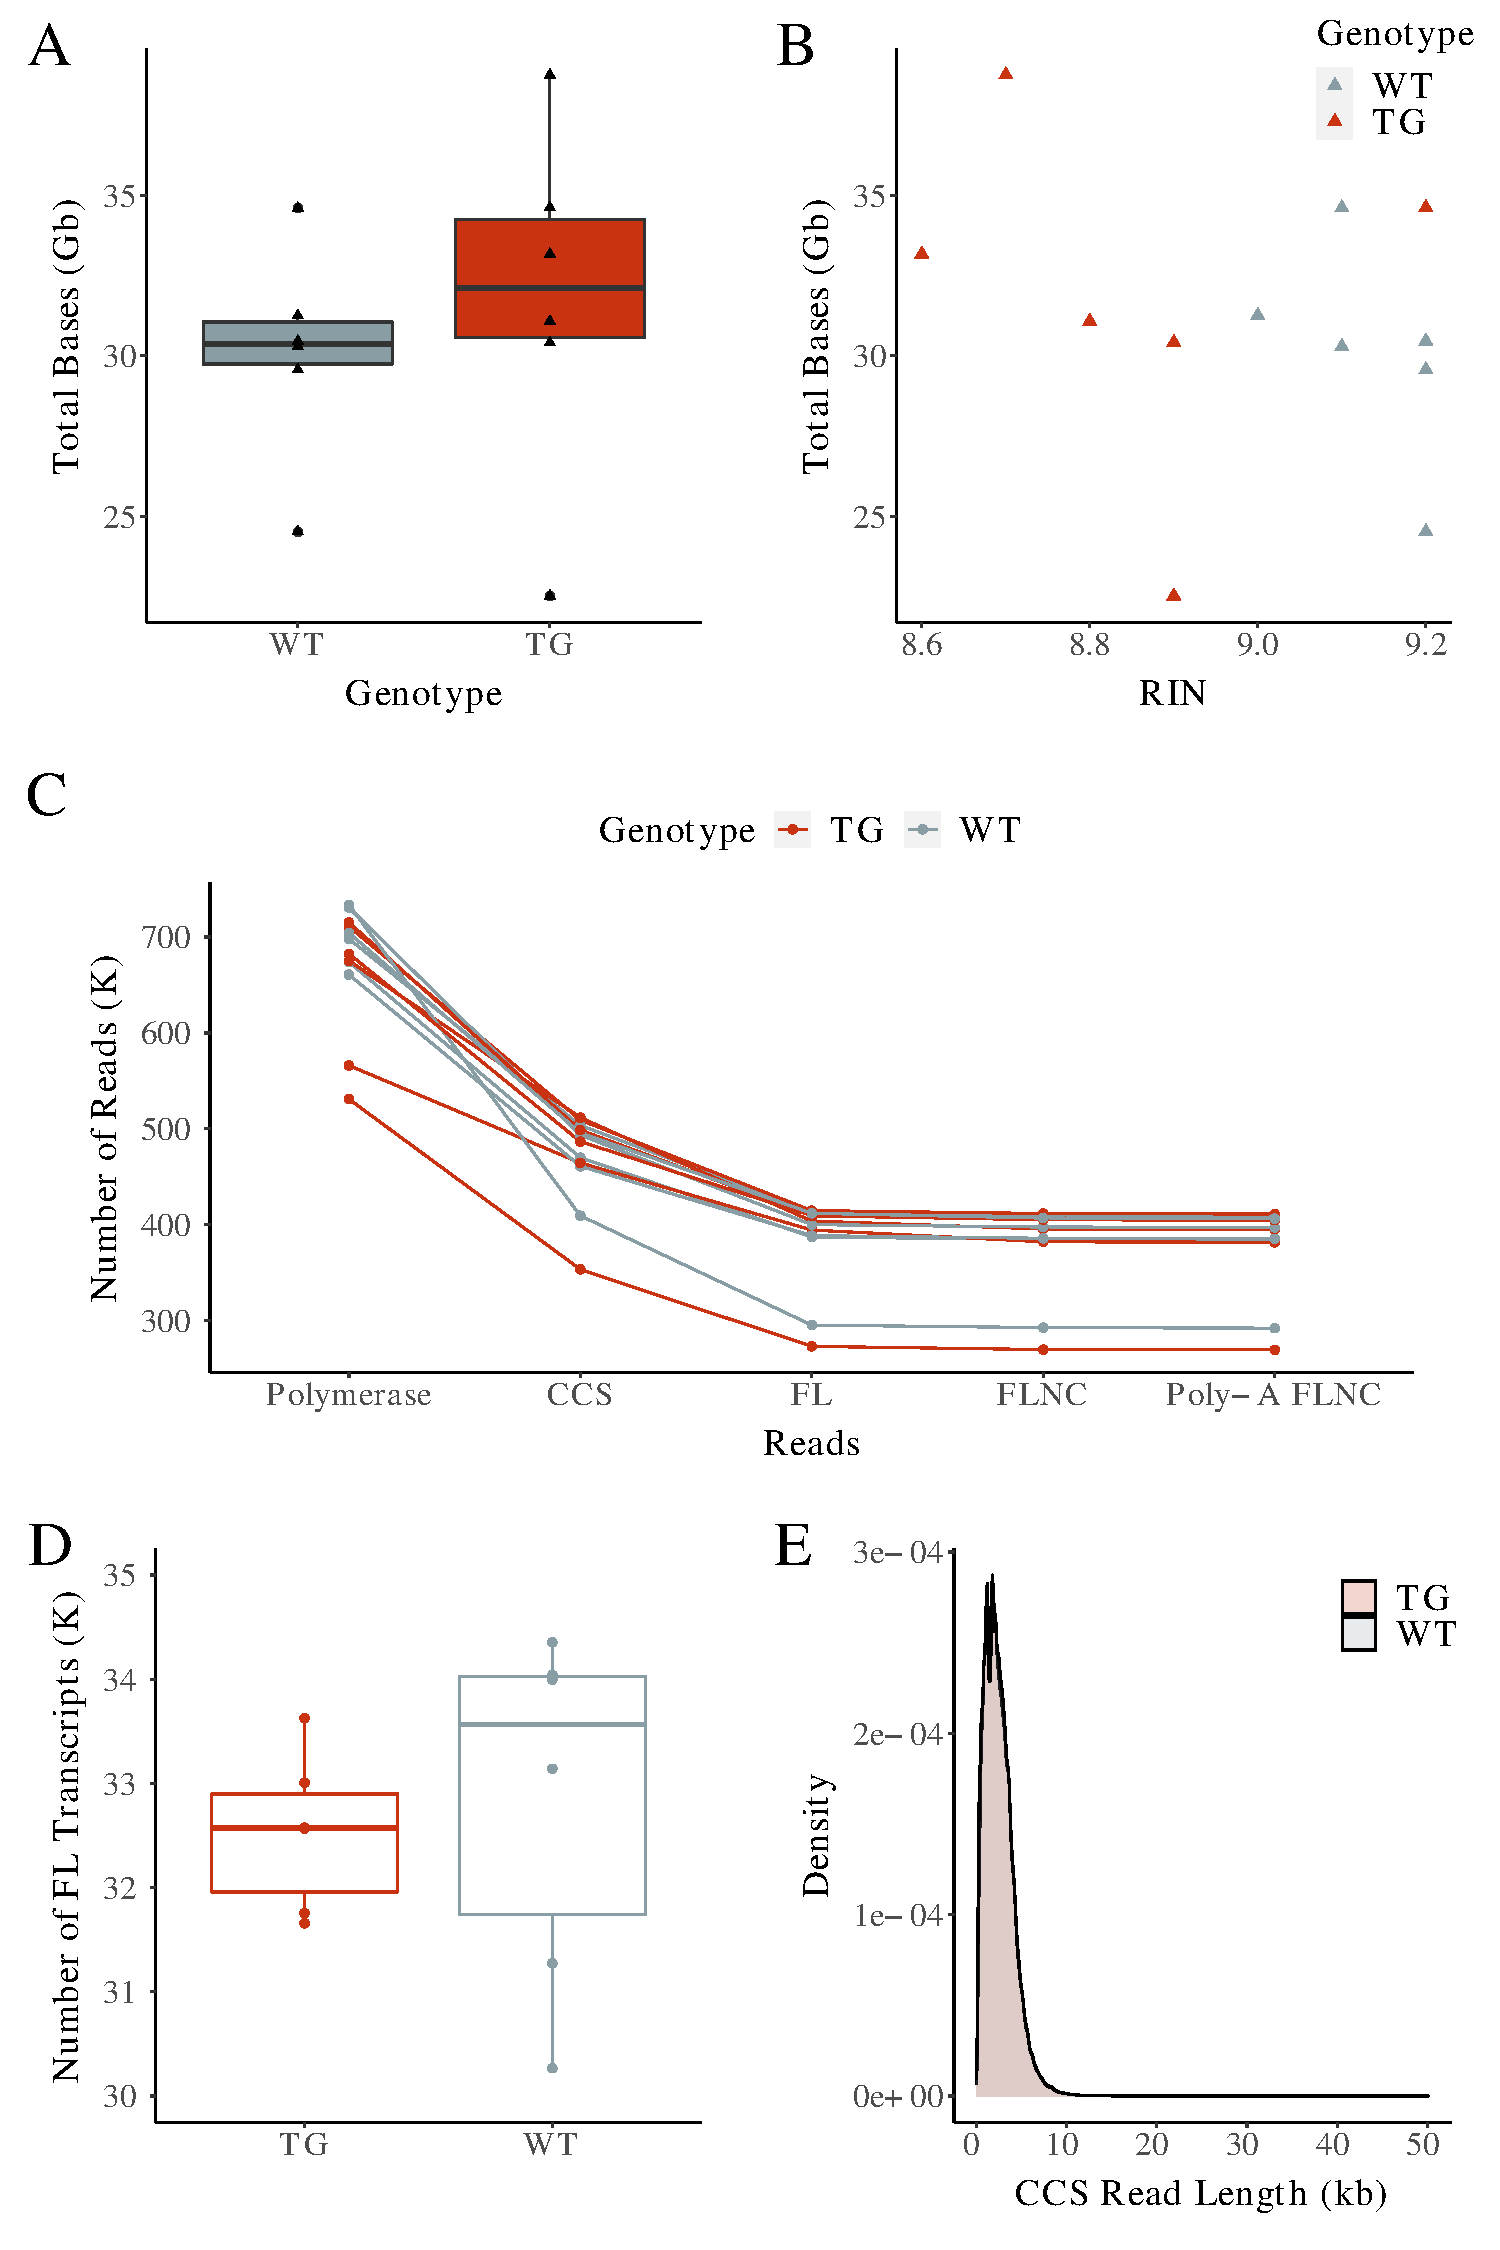
\includegraphics[page=1,trim={0 0 0 0},clip,scale = 0.55]{Figures/rTg4510WholeTranscriptome.pdf}
	\end{center}
	\captionsetup{width=0.95\textwidth}
	\caption[Sequencing and data processing metrics of rTg4510 mice]%
	{\textbf{No significant difference in sequencing metrics, number of transcripts and read length were observed between WT and rTg4501 TG mice}: \textit{Caption continues on the following page.}}
	\label{fig:rTg4510_sequencing_metrics}
\end{figure}
\begin{figure}[p]
	\captionsetup{width=0.95\textwidth}
	\caption*{\textbf{(A)} Shown is a box-plot of the total yield generated from Iso-Seq sequencing of rTg4510 WT (n = 6) and TG mice (n = 6). Full details of all runs are provided in \cref{tab:isoseq_wholerun_result}. \textbf{(B)} A scatter plot of the total yield generated and the RIN attained for each sample (RIN refers to the quality of RNA used for library preparation). \textbf{(C)} The number of reads generated through the Iso-Seq bioinformatics pipeline from initial generation of CCS reads, to FL reads with primer removal, and poly-A FLNC reads with removal of artificial concatemers and trimming of poly(A) tails. Note, the first two samples with lower throughput were sequenced with an older chemistry. \textbf{(D)} A box-plot of the total number of FL transcripts generated for WT and TG samples. \textbf{(E)} Distribution of CCS read length. CCS - Circular Consensus Sequence, FL - Full-length, FLNC - Full-length non-chimeric, Gb - Gigabases, K - Thousand, kb - Kilobases, TG - Transgenic, WT - Wild-type}%
\end{figure}


\subsection{\textit{MAPT} transgene only expressed in rTg4510 TG mice}
\label{mapt_transgene_whole}
%Check whether overexpression of human MAPT result in any unwanted, compensatory effects on equivalent mouse genes,as expression levels of mouse APP and MAPT should be slightly reduced, thereby suggesting no evidence that human transgene expression increase expression of directly-related mouse genes.
As expected, human-specific \textit{MAPT} sequences were only detected in reads from TG mice, confirming stable activation of the human \textit{MAPT} transgene (\cref{fig:isoseq_humanmapt}\textbf{A}) and supporting our previous analysis using short-read RNA-seq C\cite{Castanho2020}. Alignment of these human-specific transcripts to the mouse genome were either mapped to the mouse prion protein gene (\textit{Prnp}) with high identity but low coverage/alignment length (\cref{fig:isoseq_humanmapt}\textbf{B,C}) or to the mouse \textit{Mapt} gene with low identity but high alignment length (\cref{fig:isoseq_humanmapt}\textbf{B,D}); this is reflective of the transgene sequence in rTg4510 mouse model, given it contains exons 2 and 3 of mouse \textit{Prnp}\cite{Ramsden2005} and is homologous to the mouse \textit{Mapt} gene. Notably, applying filter thresholds (85\% alignment identity and 95\% alignment length) for downstream analysis removed these human-specific \textit{MAPT} transcripts (\cref{fig:isoseq_humanmapt}\textbf{B}). 

\begin{figure}[htp]
	\begin{center}
		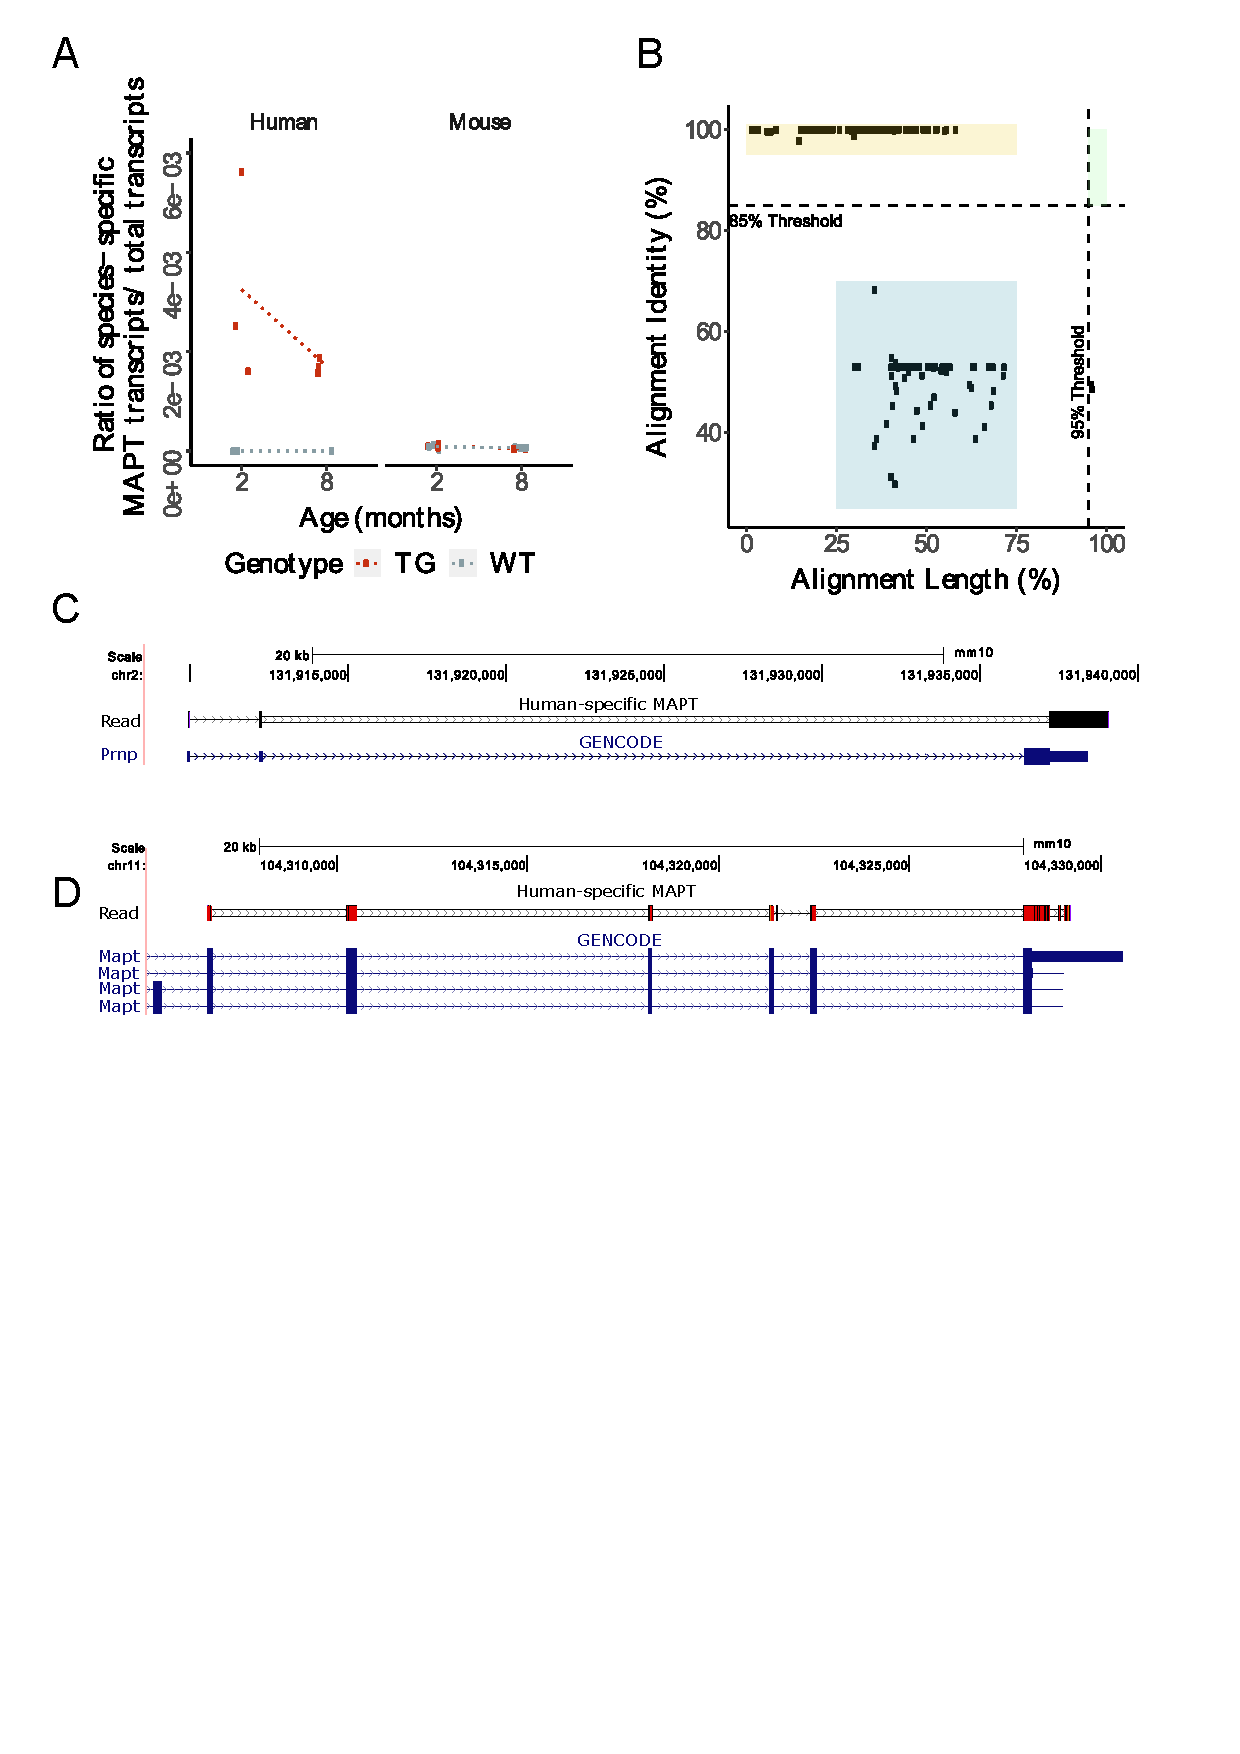
\includegraphics[page=1,trim={0cm 11cm 0cm 0cm},clip,scale = 0.80]{Figures/AltFigures_Diff.pdf}	\end{center}
	\captionsetup{width=0.95\textwidth}
	\caption[Quantifying human-specific and mouse-specific \textit{MAPT}/\textit{Mapt} sequences in Iso-Seq Whole Transcriptome]%
	{\textbf{Human-specific \textit{MAPT} sequences only present in transgenic mice with poor alignment to mouse \textit{Prnp} and \textit{Mapt} gene}: Presence of human- and mouse-specific \textit{MAPT}/\textit{Mapt} sequences was determined in full-length transcripts generated from Iso-Seq merged dataset. \textbf{(A)} Ratio of full-length transcripts that were mapped to human-specific \textit{MAPT} and mouse-specific \textit{Mapt} sequences. Dotted lines represent the mean paths across ages. \textbf{(B)} Human-specific \textit{MAPT} transcripts were poorly aligned to mouse genome, as expected. Transcripts were either aligned to mouse \textit{Prnp} gene with high identity but low length, given that the transgenic contains only exon 2 and 3 of mouse \textit{Prnp} gene\cite{Ramsden2005} (boxed yellow) or  mouse \textit{Mapt} gene with low alignment identity and length (boxed blue). Green box refers to the transcripts retained after applying identity and length threshold. \textbf{(C)} USCS genome browser tracks of human-specific (black) \textit{MAPT} transcripts (transgene) and mouse \textit{Prnp} gene and \textbf{(D)} mouse \textit{Mapt} gene. Blue tracks represent known transcripts from reference mouse genome (mm10). The double horizontal lines indicate unalignable sequences and the red lines indicate bases that deter between the genome and read. Tracks were cropped and modified to remove irrelevant genes within the same locus.  UTR - Untranslated region}
	\label{fig:isoseq_humanmapt}
\end{figure}

\clearpage
\subsection{rTg4510 TG mice are characterised by a similar global transcriptomic profile to WT mice}
Despite identifying widespread RNA isoform diversity amongst genes expressed in the mouse entorhinal cortex (\cref{ch: whole_transcriptome}), the global transcriptomic profile between rTg4510 WT and TG mice were very similar; no difference was observed in the number of genes (mean number = 13,572 genes) or isoforms (mean number = 53,833 isoforms). Further characterisation of the transcriptome revealed similar profile of isoform diversity across genotype and age (\cref{tab:isoseq_whole_subsqantioutput}), with half of the isoforms annotated as known and FSM (mean number = 30,018 isoforms (55.8\%), as also shown in \cref{sec:whole_novelIso}) and with a similar distribution of isoform length and exon number (median = 8, range = 1-89). Splicing patterns were also very similar across genotype and age with usage of alternative first exons (AF) (mean n = 12,564, 35\%) (\cref{AS_WholeTranscriptome_diff}) as the most prevalent across all datasets, in line with previous findings (\cref{sec:whole_novelIso}).

\vspace{2cm}
\begin{table}[!htp]
	\centering
	\captionsetup{width=1\textwidth}
	\caption[Alternative Splicing Events associated with tau pathology and age]%
	{\textbf{Alternative Splicing Events associated with tau pathology and age}. Tabulated is the number of splicing events detected for wild-type and transgenic Tg4510 mice aged 2 and 8 months (n = 12, 3 biological replicates per group)}
	\begin{tabular}{@{}ccccc@{}}
		\toprule
		\multirow{2}{*}{Splicing  Events} & \multicolumn{2}{c}{Wildtype} & \multicolumn{2}{c}{Transgenic} \\ \cmidrule(l){2-5} 
		& 2 months        & 8 months        & 2 months        & 8 months        \\ \midrule
		A3 & 2164 (6.58\%)   & 2571 (6.61\%)   & 2388 (6.77\%)   & 2388 (6.5\%)    \\
		A5 & 1369 (4.16\%)   & 1589 (4.09\%)   & 1473 (4.18\%)   & 1488 (4.05\%)   \\
		AF & 12048 (36.61\%) & 13073 (33.61\%) & 12514 (35.48\%) & 12622 (34.36\%) \\
		AL & 8140 (24.73\%)  & 9688 (24.91\%)  & 8641 (24.5\%)   & 9287 (25.28\%)  \\
		IR & 3611 (10.97\%)  & 5404 (13.9\%)   & 4293 (12.17\%)  & 4774 (13\%)     \\
		MX & 299 (0.91\%)    & 392 (1.01\%)    & 331 (0.94\%)    & 329 (0.9\%)     \\
		SE & 5278 (16.04\%)  & 6174 (15.88\%)  & 5632 (15.97\%)  & 5846 (15.91\%)  \\ \bottomrule
	\end{tabular}
	\label{AS_WholeTranscriptome_diff}
\end{table}

%stats?
%XX of known transcripts were identified to have intron retention; XX of known transcripts were identified to be fusion genes. XX of know transcripts identified to have non-sense-mediated decay. 

\begin{landscape}
	\begin{table}[]
		\centering
		\captionsetup{width=1\linewidth}
		\caption[Overview of the whole transcriptome Iso-Seq datasets generated from mouse rTg4510, subsected by phenotype and age]%
		{\textbf{Overview of the whole transcriptome Iso-Seq datasets generated from mouse rTg4510, subsected by phenotype and age}. Annotations from wild-type (n = 6) and transgenic mouse (n = 6) were generated from merging Iso-Seq datasets from mouse aged 2 and 8 months of the respective phenotype. Novel genes refer to genes that were not currently present in existing genome annotations (mm10). Isoform can be further classified as known (FSM, ISM) or novel (ISM, NIC, NNC, Genic Genomic, Antisense, Fusion, Intergenic, Genic Intron), as described in \cref{sec:sq_exp}. FSM – Full Splice Match, ISM – Incomplete Splice Match, NIC – Novel In Catalogue, NNC – Novel Not in Catalogue.}
		\label{tab:isoseq_whole_subsqantioutput}
		\resizebox{1.5\textwidth}{!}{%
		\begin{tabular}{@{}ccccccc@{}}
		\toprule
		\multicolumn{1}{l}{} &
		\begin{tabular}[c]{@{}c@{}}Wildtype \\ (n = 6)\end{tabular} &
		\begin{tabular}[c]{@{}c@{}}Transgenic \\ (n = 6)\end{tabular} &
		\begin{tabular}[c]{@{}c@{}}Wildtype, 2 months \\ ( n = 3)\end{tabular} &
		\begin{tabular}[c]{@{}c@{}}Wildtype, 8 months \\ ( n = 3)\end{tabular} &
		\begin{tabular}[c]{@{}c@{}}Transgenic, 2 months\\ ( n = 3)\end{tabular} &
		\begin{tabular}[c]{@{}c@{}}Transgenic, 8 months \\ ( n = 3)\end{tabular} \\ \midrule
		Total Number of Genes             & 14118           & 14213           & 13191           & 13312           & 12985           & 13616           \\
		Annotated Genes                   & 13932 (98.68\%) & 14031 (98.72\%) & 13081 (99.17\%) & 13168 (98.92\%) & 12874 (99.15\%) & 13474 (98.96\%) \\
		Novel Genes                       & 186 (1.32\%)    & 182 (1.28\%)    & 110 (0.83\%)    & 144 (1.08\%)    & 111 (0.85\%)    & 142 (1.04\%)    \\
		Total Number of Isoforms          & 62533           & 63038           & 48516           & 50278           & 45903           & 52730           \\
		FSM                               & 33239 (53.15\%) & 33563 (53.24\%) & 27878 (57.46\%) & 28689 (57.06\%) & 26825 (58.44\%) & 29916 (56.73\%) \\
		ISM                               & 4927 (7.88\%)   & 4864 (7.72\%)   & 3426 (7.06\%)   & 3841 (7.64\%)   & 3279 (7.14\%)   & 3764 (7.14\%)   \\
		NIC                               & 15305 (24.48\%) & 15595 (24.74\%) & 11012 (22.7\%)  & 11407 (22.69\%) & 10214 (22.25\%) & 12369 (23.46\%) \\
		NNC                               & 8518 (13.62\%)  & 8484 (13.46\%)  & 5838 (12.03\%)  & 5953 (11.84\%)  & 5259 (11.46\%)  & 6282 (11.91\%)  \\
		Genic Genomic                     & 63 (0.1\%)      & 61 (0.1\%)      & 44 (0.09\%)     & 44 (0.09\%)     & 32 (0.07\%)     & 47 (0.09\%)     \\
		Antisense                         & 97 (0.16\%)     & 104 (0.16\%)    & 52 (0.11\%)     & 77 (0.15\%)     & 68 (0.15\%)     & 75 (0.14\%)     \\
		Fusion                            & 276 (0.44\%)    & 268 (0.43\%)    & 200 (0.41\%)    & 186 (0.37\%)    & 167 (0.36\%)    & 196 (0.37\%)    \\
		Intergenic                        & 108 (0.17\%)    & 99 (0.16\%)     & 66 (0.14\%)     & 81 (0.16\%)     & 59 (0.13\%)     & 81 (0.15\%)     \\
		Genic Intron                      & 0 (0\%)         & 0 (0\%)         & 0 (0\%)         & 0 (0\%)         & 0 (0\%)         & 0 (0\%)         \\
		Isoform Length (bp) &
		\begin{tabular}[c]{@{}c@{}}Median: 2691, \\ Range: 82-15016\end{tabular} &
		\begin{tabular}[c]{@{}c@{}}Median: 2698, \\ Range: 82-15913\end{tabular} &
		\begin{tabular}[c]{@{}c@{}}Median: 2740, \\ Range: 88-15016\end{tabular} &
		\begin{tabular}[c]{@{}c@{}}Median: 2614, \\ Range: 82-14850\end{tabular} &
		\begin{tabular}[c]{@{}c@{}}Median: 2548, \\ Range: 88-14302\end{tabular} &
		\begin{tabular}[c]{@{}c@{}}Median: 2754, \\ Range: 82-15913\end{tabular} \\
		Number of Exons &
		\begin{tabular}[c]{@{}c@{}}Median: 8, \\ Range: 1-89\end{tabular} &
		\begin{tabular}[c]{@{}c@{}}Median: 8, \\ Range: 1-89\end{tabular} &
		\begin{tabular}[c]{@{}c@{}}Median: 9, \\ Range: 1-89\end{tabular} &
		\begin{tabular}[c]{@{}c@{}}Median: 8, \\ Range: 1-89\end{tabular} &
		\begin{tabular}[c]{@{}c@{}}Median: 8, \\ Range: 1-77\end{tabular} &
		\begin{tabular}[c]{@{}c@{}}Median: 9, \\ Range: 1-89\end{tabular} \\
		Number of Isoforms with 50bp CAGE & 52096 (83.31\%) & 52633 (83.49\%) & 40589 (83.66\%) & 42378 (84.29\%) & 38227 (83.28\%) & 44729 (84.83\%) \\ \bottomrule
	\end{tabular}%
		}
		\end{table}
\end{landscape}

 
\subsection{Iso-Seq confirms widespread gene expression differences associated with tau pathology in rTg4510 mice detected using short-read RNA-seq}
\label{ch5: diffgeneexp}
%\boldheader{Usage of Iso-Seq reads alone detected robust changes in gene expression}
Although long-read sequencing is often assumed to be less quantitative than traditional short-read RNA sequencing approaches, we previously demonstrated the power of Iso-Seq to accurately quantify the abundance of highly-expressed transcripts (described in \cref{sec: whole_isoseqvsrnaseq}). Subsequently, we sought to evaluate the utility of full-length Iso-Seq read counts as a proxy of abundance to identify changes in gene expression associated with progressive tau pathology in TG mice. Of note, a recent RNA-Seq study by our group identified extensive gene expression differences in the same mouse model using short-read RNA-Seq data mapped to the mouse reference genome annotation\cite{Castanho2020}.

Using Iso-Seq reads for annotation and expression, we identified 483 genes differentially expressed at a stringent FDR < 0.05. Using \textit{MasigPro} to differentiate genotype and age effects (illustrated in \cref{fig:dea_model}), we identified evidence for differential gene expression associated with the rTg4510 genotype (\cref{fig:dea_model_genexp}\textbf{A}) and age (\cref{fig:dea_model_genexp}\textbf{B}), and also genes expression interactions between genotype and age (\cref{fig:dea_model_genexp}\textbf{D,E,F,G}). Classifying differentially expressed genes by effects, we identified 18 differentially expressed genes that were associated by genotype effect and 356 genes (73.7\%) genes whose expression significantly changed with tau pathology progression in rTg4510 mice (\cref{fig:dea_model_num}). Among these, there was a significant (exact bionomial test, n = 356 genes, P = 1.91 x 10\textsuperscript{-44}) enrichment of upregulated genes (n = 304 genes (85.3\%) with upregulated expression in TG compared to WT; n = 52 (14.6\%) genes with downregulated expression in TG). Using \textit{EnrichR}, the differentially expressed genes were found to be highly enriched in the lysosome (GO Cellular Component: odds ratio = 3.06, adjusted p-value= 4.19 x 10\textsuperscript{-4}) and in particularly the TGF-\textbeta signalling pathway (WikiPathway 2021 Human: odds ratio = 17.16, adjusted p-value= 2.92 x 10\textsuperscript{-2} ). Further in line with previous findings, a third of genes identified with expression changes from Iso-Seq reads were enriched in pathways involved in immune system activation (n = 140 genes, 34.4\%, "turquoise" co-expression module\cite{Castanho2020}, \cref{fig:dea_model_num}\textbf{B}). 

Our previous RNA-Seq study\cite{Castanho2020} was more powered with a bigger sample size (RNA-Seq: n = 29 rTg4510 TG, n = 30 WT; Iso-Seq: n = 6 TG, n = 6 WT) and deeper sequencing coverage (RNA-Seq: mean number of reads = 18.8M; Iso-Seq: mean number of CCS reads = 5.7M reads) and unsurprisingly identified a larger number of gene expression changes (n = 1916 differentially expressed genes). Of note, 116 (6.05\%) of these genes were also detected as differentially expressed using normalised Iso-Seq read counts. Unsurprisingly, the results derived from normalised RNA-Seq counts aligned to the reference genome and the improved Iso-Seq-derived transcriptome annotations were more concurrent (n = 841 common differentially expressed genes, 43.9\%). Using normalised Iso-Seq read counts as proxy of expression, the top differentially expressed gene associated with progressive tau pathology rTg4510 mice was also \textit{Gfap} - which encodes for glial fibrillary acidic protein (GFAP\nomenclature{GFAP}{Glial Fibrillary Acidic Protein}), a cytoskeletal protein that acts as a marker for astrocyte activation and its upregulation in human AD post-mortem brain tissues and other AD mouse  models has been well reported\cite{Muramori1998,Ishiki2016, Chatterjee2021}. Other top-ranked tau-associated differentially-expressed genes (\cref{tab:dea_wholemouse}) have been previously reported to play a role in AD development and pathology, notably \textit{C4b}\cite{Zorzetto2016} - a member of the complement immune system (\cref{fig:whole_dea}\textbf{C,D}), \textit{Slc14a1}\cite{Castillo2017} encoding the urea transporter 1, \textit{Tgfbr1} encoding the TGF-\textbeta receptor protein (\cref{fig:whole_dea}\textbf{E,F}) and \textit{Unc93b1}\cite{Wirz2013}, a transmembrane protein required for toll (\cref{tab:dea_wholemouse}). 

  
\begin{figure}[h]
	\centering
	\includegraphics[page=5,scale = 0.55]{Figures/WholeDifferentialAnalysis.pdf}
	\captionsetup{width=0.95\textwidth}
	\caption[Examples of gene expression differing across conditions]%
	{\textbf{Differential expressed genes exhibiting genotype, age and interaction effects} Shown are examples of differentially expressed genes classified under the different models, using the whole transcriptome dataset (WT = 6, TG = 6, across age 2 and 8 months) using Iso-Seq read counts as abundance: \textbf{(A)} \textit{Tigd2} with a genotype effect, \textbf{(B)} \textit{Mobp} with a genotype and age effect, \textbf{(C)} \textit{Cik1} with an age effect, and \textbf{(D)} \textit{Cd34}, \textbf{(E)} \textit{Unc93b1}, \textbf{(F)} \textit{Csf1r} and \textbf{(G)} \textit{Tgfbr2} with an interaction effect. Dashed lines represent mean paths across age groups. rTg4510 wild-type and transgenic mice are denoted by red and grey, respectively. }   
	\label{fig:dea_model_genexp}
\end{figure}
 
\begin{figure}[h]
	\centering
	\includegraphics[page=4,trim={0 19cm 0 0},clip,scale = 0.55]{Figures/WholeDifferentialAnalysis.pdf}
	\captionsetup{width=0.95\textwidth}
	\caption[Differentially expressed genes classified by conditions]%
	{\textbf{Differentially expressed genes were identified across all the different conditions with a number of differentially expressed genes exhibiting an interaction effect of rTg4510 genotype and age.} \textbf{(A)} A bar plot of the number of differentially expressed genes (n = 483, determined from Iso-Seq FL read count as proxy of expression) classified by rTg4510 genotype, age, and interaction effect (n = 6 WT, n = 6 TH, across 2 and 8 months). \textbf{(B)} A pie chart of the number and proportion of differentially expressed genes with genotype and interaction effect (n = 407 genes) identified in discrete co-expression network modules from a previous RNA-Seq study\cite{Castanho2020}; all three modules are significantly associated with progressive tau pathology: "Red" module is downregulated in TG and enriched in synaptic transmission, "Turquoise" module is upregulated in TG and enriched for immune system activation, and "Yellow" module is downregulated in TG and enriched in mitochondria and synpatic processes.}    
	\label{fig:dea_model_num}
\end{figure}


\begin{figure}[h]
	\begin{center}
		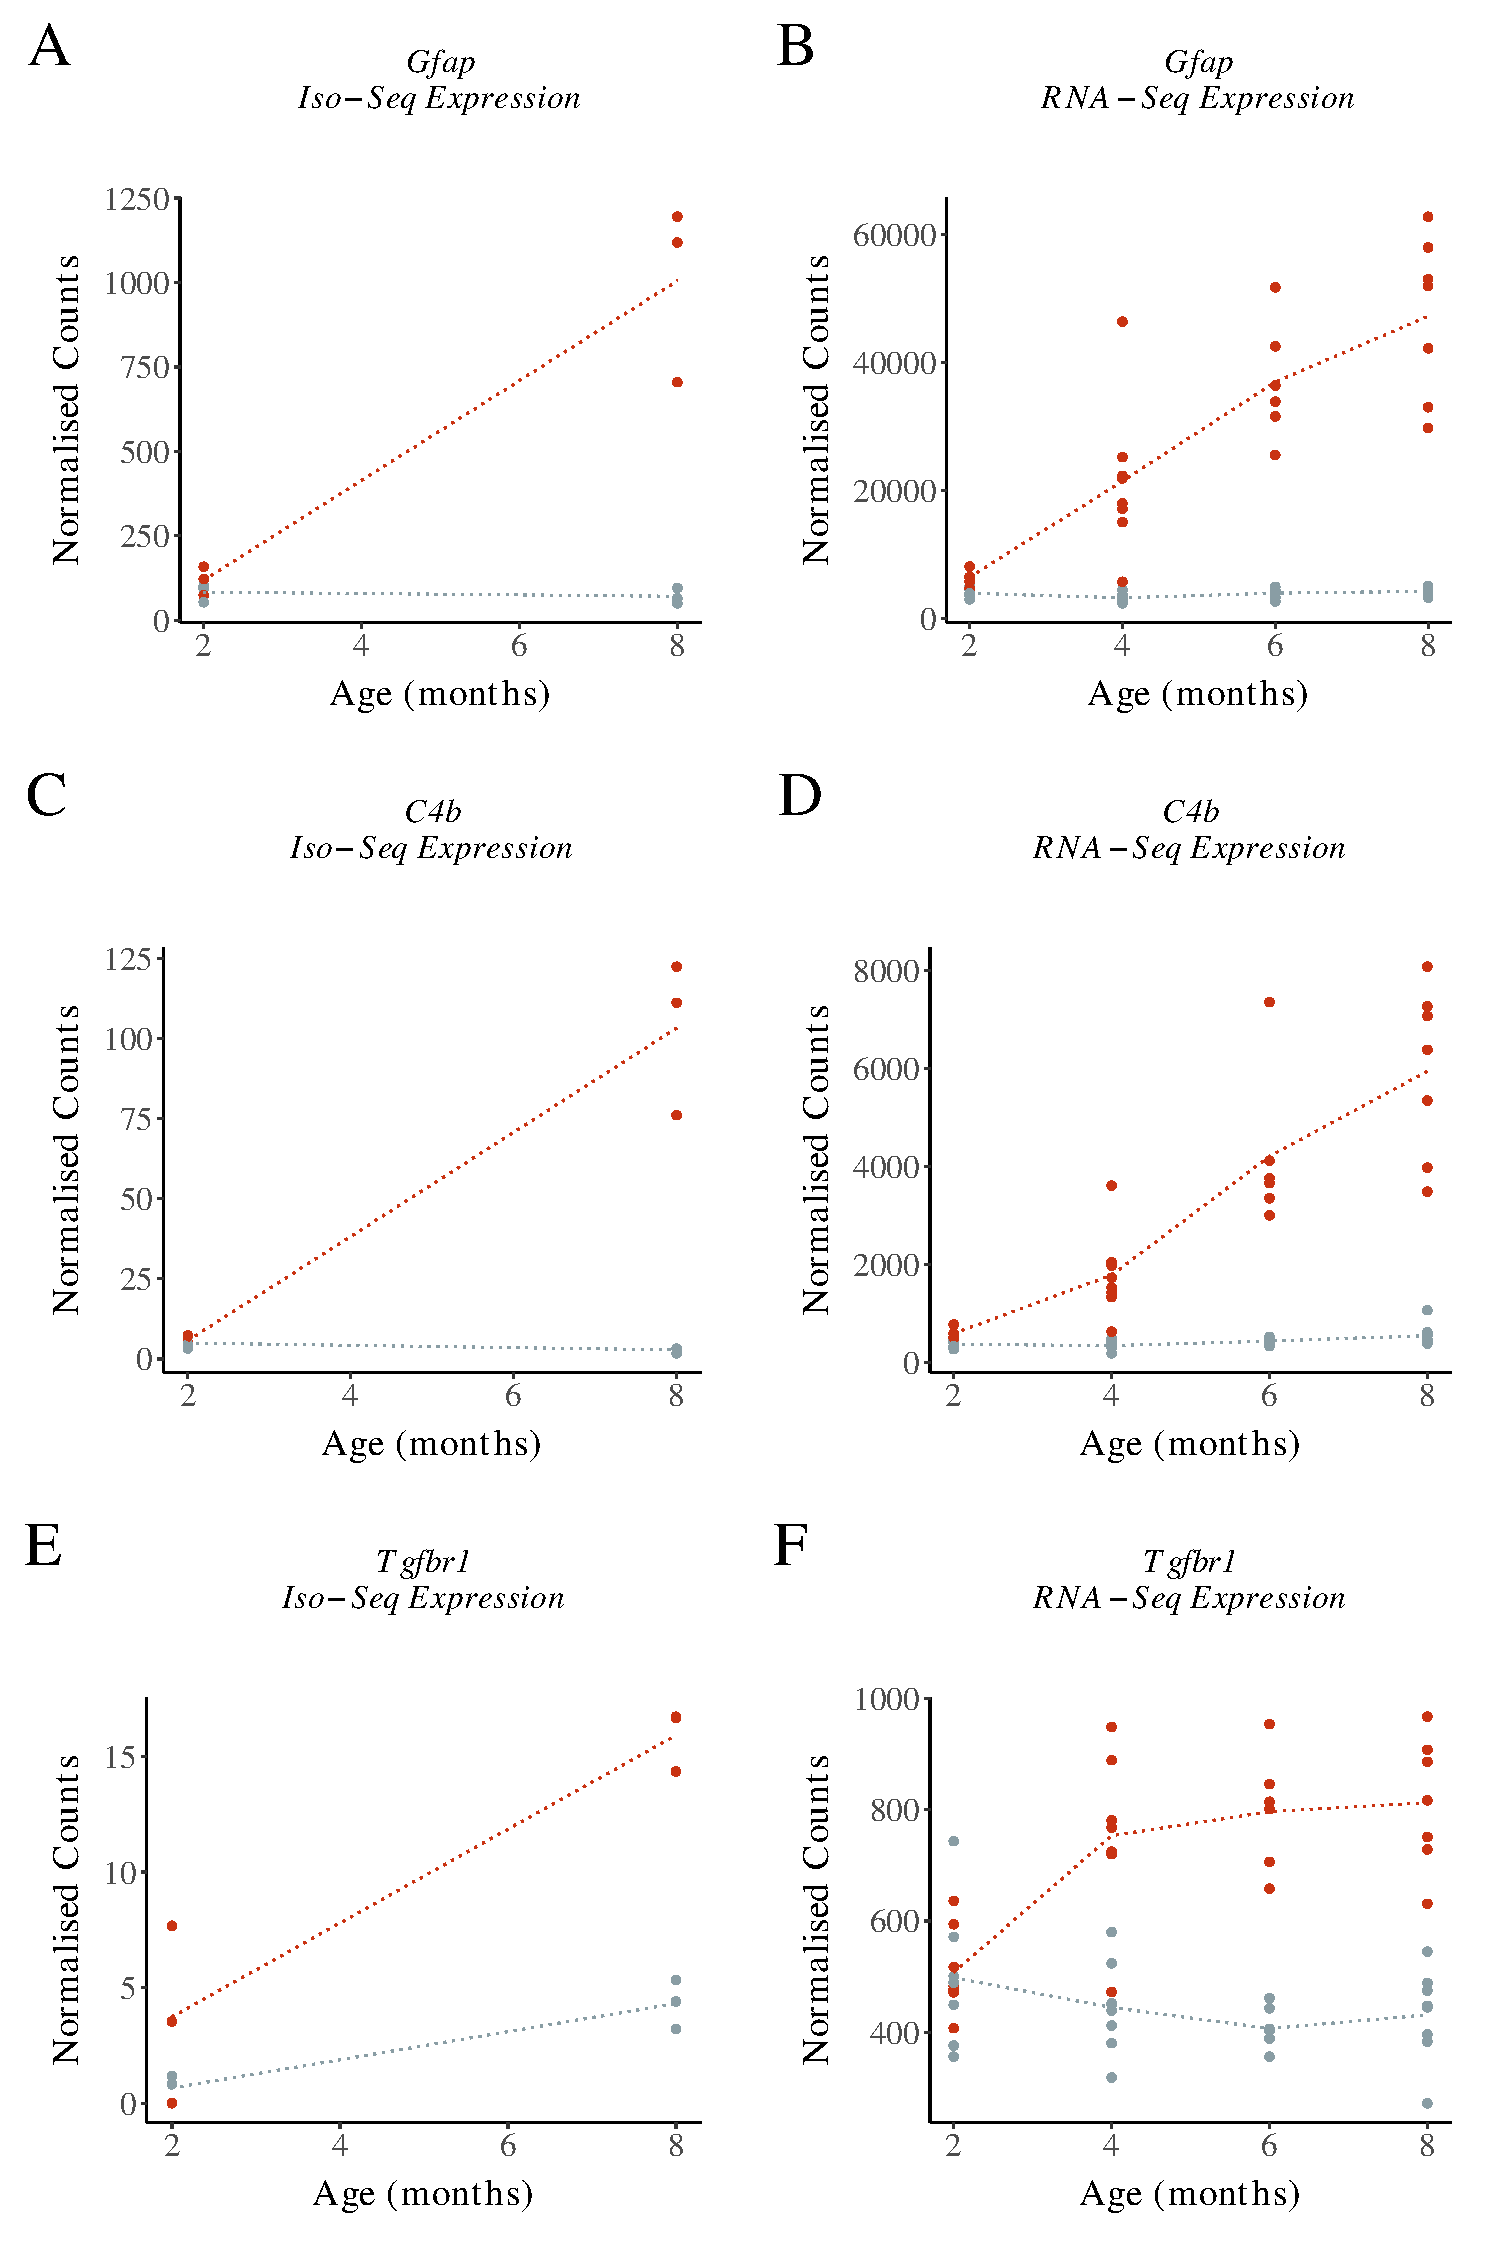
\includegraphics[page=1,scale = 0.55]{Figures/WholeDifferentialAnalysis.pdf}
	\end{center}
	\captionsetup{width=0.95\textwidth}
	\caption[Top ranked differentially expressed genes associated with progressive tau pathology in rTg4510]%
	{\textbf{Top ranked differentially expressed genes associated with progressive tau pathology in rTg4510}: Shown are the the expression plots for \textbf{(A, B)} \textit{Gfap}, \textbf{(C, D)} \textit{C4b} and \textbf{(E, F)} \textit{Tgfbr1} using either Iso-Seq FL read count or RNA-Seq reads as expression. Dashed lines represent mean paths across age groups. rTg4510 wild-type and transgenic mice are denoted by red and grey, respectively.}   
	\label{fig:whole_dea}
\end{figure}

\vspace{2cm}
%log2fc calculated by mean expression at 8 case/mean expression at 8 control
\begin{table}[!htp]
	\centering
	\caption[Top-ranked differentially expressed genes associated with rTg4510 genotype]%
	{Tabulated are the top-ranked genes identified as differentially expressed in rTg4510 transgenic mice using \textit{maSigPro} with Iso-Seq defined transcriptome for annotation and Iso-Seq FL read count as expression. Gene expression is determined from the sum of normalised expression of associated transcripts. FDR - False Discovery Rate. }
	\begin{tabularx}{0.85\textwidth}{cccccccc}
	\toprule
	\multirow{3}{*}{Gene} &
	\multirow{3}{*}{FDR} &
	\multirow{3}{*}{R\textsuperscript{2}} &
	\multirow{3}{*}{\begin{tabular}[c]{@{}c@{}}log2-fold\\  change \\ (8 months)\end{tabular}} &
	\multicolumn{4}{c}{Mean Gene Expression} \\ \cmidrule(l){5-8} 
	&          &       &      & \multicolumn{2}{c}{Wild-type} & \multicolumn{2}{c}{Transgenic} \\ \cmidrule(l){5-8} 
	&          &       &      & 2 moss      & 8 mos      & 2 mos       & 8 mos      \\ \midrule
	\textit{C4b}    & 1.6 x 10\textsuperscript{-41}  & 0.945 & 4.38 & 4.94          & 2.73          & 4.97           & 103           \\
	\textit{Gfap}     & 6.04 x 10\textsuperscript{-36} & 0.933 & 3.12  & 82.8          & 70.5          & 118            & 1030           \\
	\textit{Tgfbr1}  & 7.9 x 10\textsuperscript{-24}  & 0.892 & 2.95 & 0.663         & 3.38          & 2.03           & 15.7          \\
	\textit{Slc14a1} & 4.31 x 10\textsuperscript{-22} & 0.899 & 2.95 & 9.55          & 14.7          & 6.16           & 47.7            \\
	\textit{Pros1} & 1.05 x 10\textsuperscript{-17} & 0.894 & 2.08 & 8.17          & 9.32         & 6.26           & 26.4          \\
	\textit{Unc93b1} & 1.46 x 10\textsuperscript{-16} & 0.863 & 1.61  & 3.59          & 5.04          & 6.47          & 19.8          \\ \bottomrule
	\end{tabularx}
	\label{tab:dea_wholemouse}
\end{table}

\clearpage
\subsection{rTg4510 mice characterised by expression differences in novel, antisense genes}
Highlighting the power of long-reads to comprehensively annotate the transcriptome, we previously detected novel genes in our Iso-Seq dataset that were not present in existing genome annotations(\cref{sec:whole_novelgenes}). These genes were often lowly-expressed and typically antisense to known genes with overlap at the UTR or gene body. Given the improved transcript annotation afforded by our Iso-Seq data, we next sought to test for expression changes in these novel genes associated with rTg4510 genotype, quantifying levels of expression by mapping RNA-seq reads to our reference transcriptome. 

We identified 3 of these novel genes wvidence for differential expression associated with rTg4510 genotype. The most significant differentially-expressed novel gene was located on chromosome 10 (PB.1799.1, \cref{fig:whole_novelgene_difftracks}\textbf{A}) and was characterised by progressive down-regulation in TG mice (\cref{fig:whole_novelgene_diffexp}\textbf{A}). The other two differentially-expressed novel genes were found antisense to known genes: \textit{Fgfr1op} (PB.6616.1, \cref{fig:whole_novelgene_difftracks}\textbf{B}) within the gene-body and \textit{Htra1} at the 5'UTR (PB.15002.1, \cref{fig:whole_novelgene_difftracks}\textbf{C}). Both genes were upregulated with progressive tau pathology in TG mice (\cref{fig:whole_novelgene_diffexp}\textbf{B,D}). Notably, while \textit{Fgfr1op} was not identified as differentially-expressed (\cref{fig:whole_novelgene_diffexp}\textbf{C}), \textit{Htra1} was also found to have higher expression in rTg4510 TG compared to WT (\cref{fig:whole_novelgene_diffexp}\textbf{E}).     
%Htra1-AS shared exonic regions with Htra1 so misalignment of RNA-Seq reads

\begin{landscape}
	\begin{figure}[!htp]
		\centering
		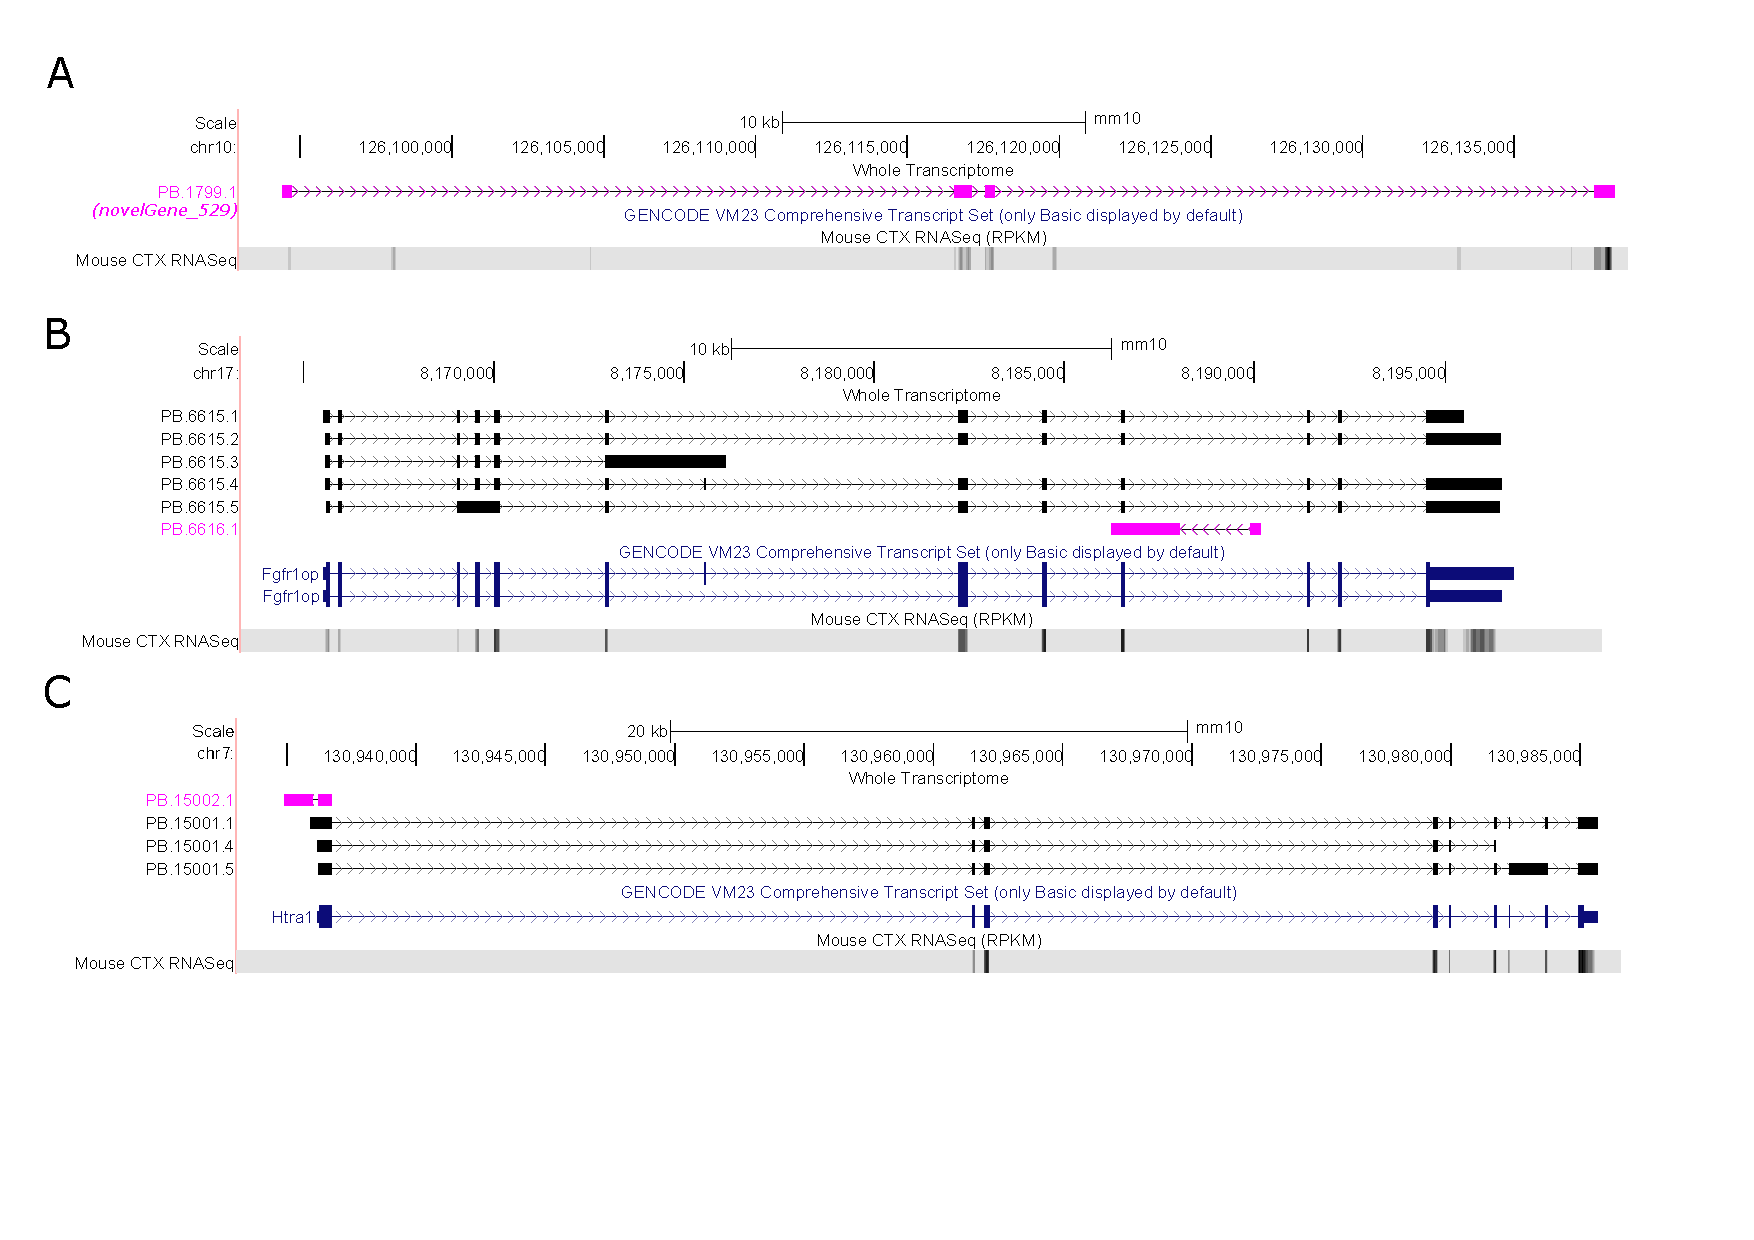
\includegraphics[page=1,trim={0 3.5cm 0 1cm}, scale = 0.80]{Figures/TracksFigures_Diff.pdf}
		\captionsetup{width=1.4\textwidth}
		\caption[Visualisation of differentially expressed novel genes in rTg4510 TG mice]%
		{\textbf{Visualisation of novel genes that were differentially expressed in rTg4510 mice.} Shown are UCSC genome browser tracks of three novel genes (coloured pink) whose expression changed with rTg4510 genotype: \textbf{(A)} novel gene in chromosome 10, \textbf{(B)} novel gene antisense to \textit{Fgfr1op}, and \textbf{(C)} novel gene antisense to \textit{Htra1}. Shown are also reference genome annotations (mm10) and RNA-Seq data from matched samples.}   
		\label{fig:whole_novelgene_difftracks}
	\end{figure}
\end{landscape}

\begin{figure}[!htp]
	\begin{center}
		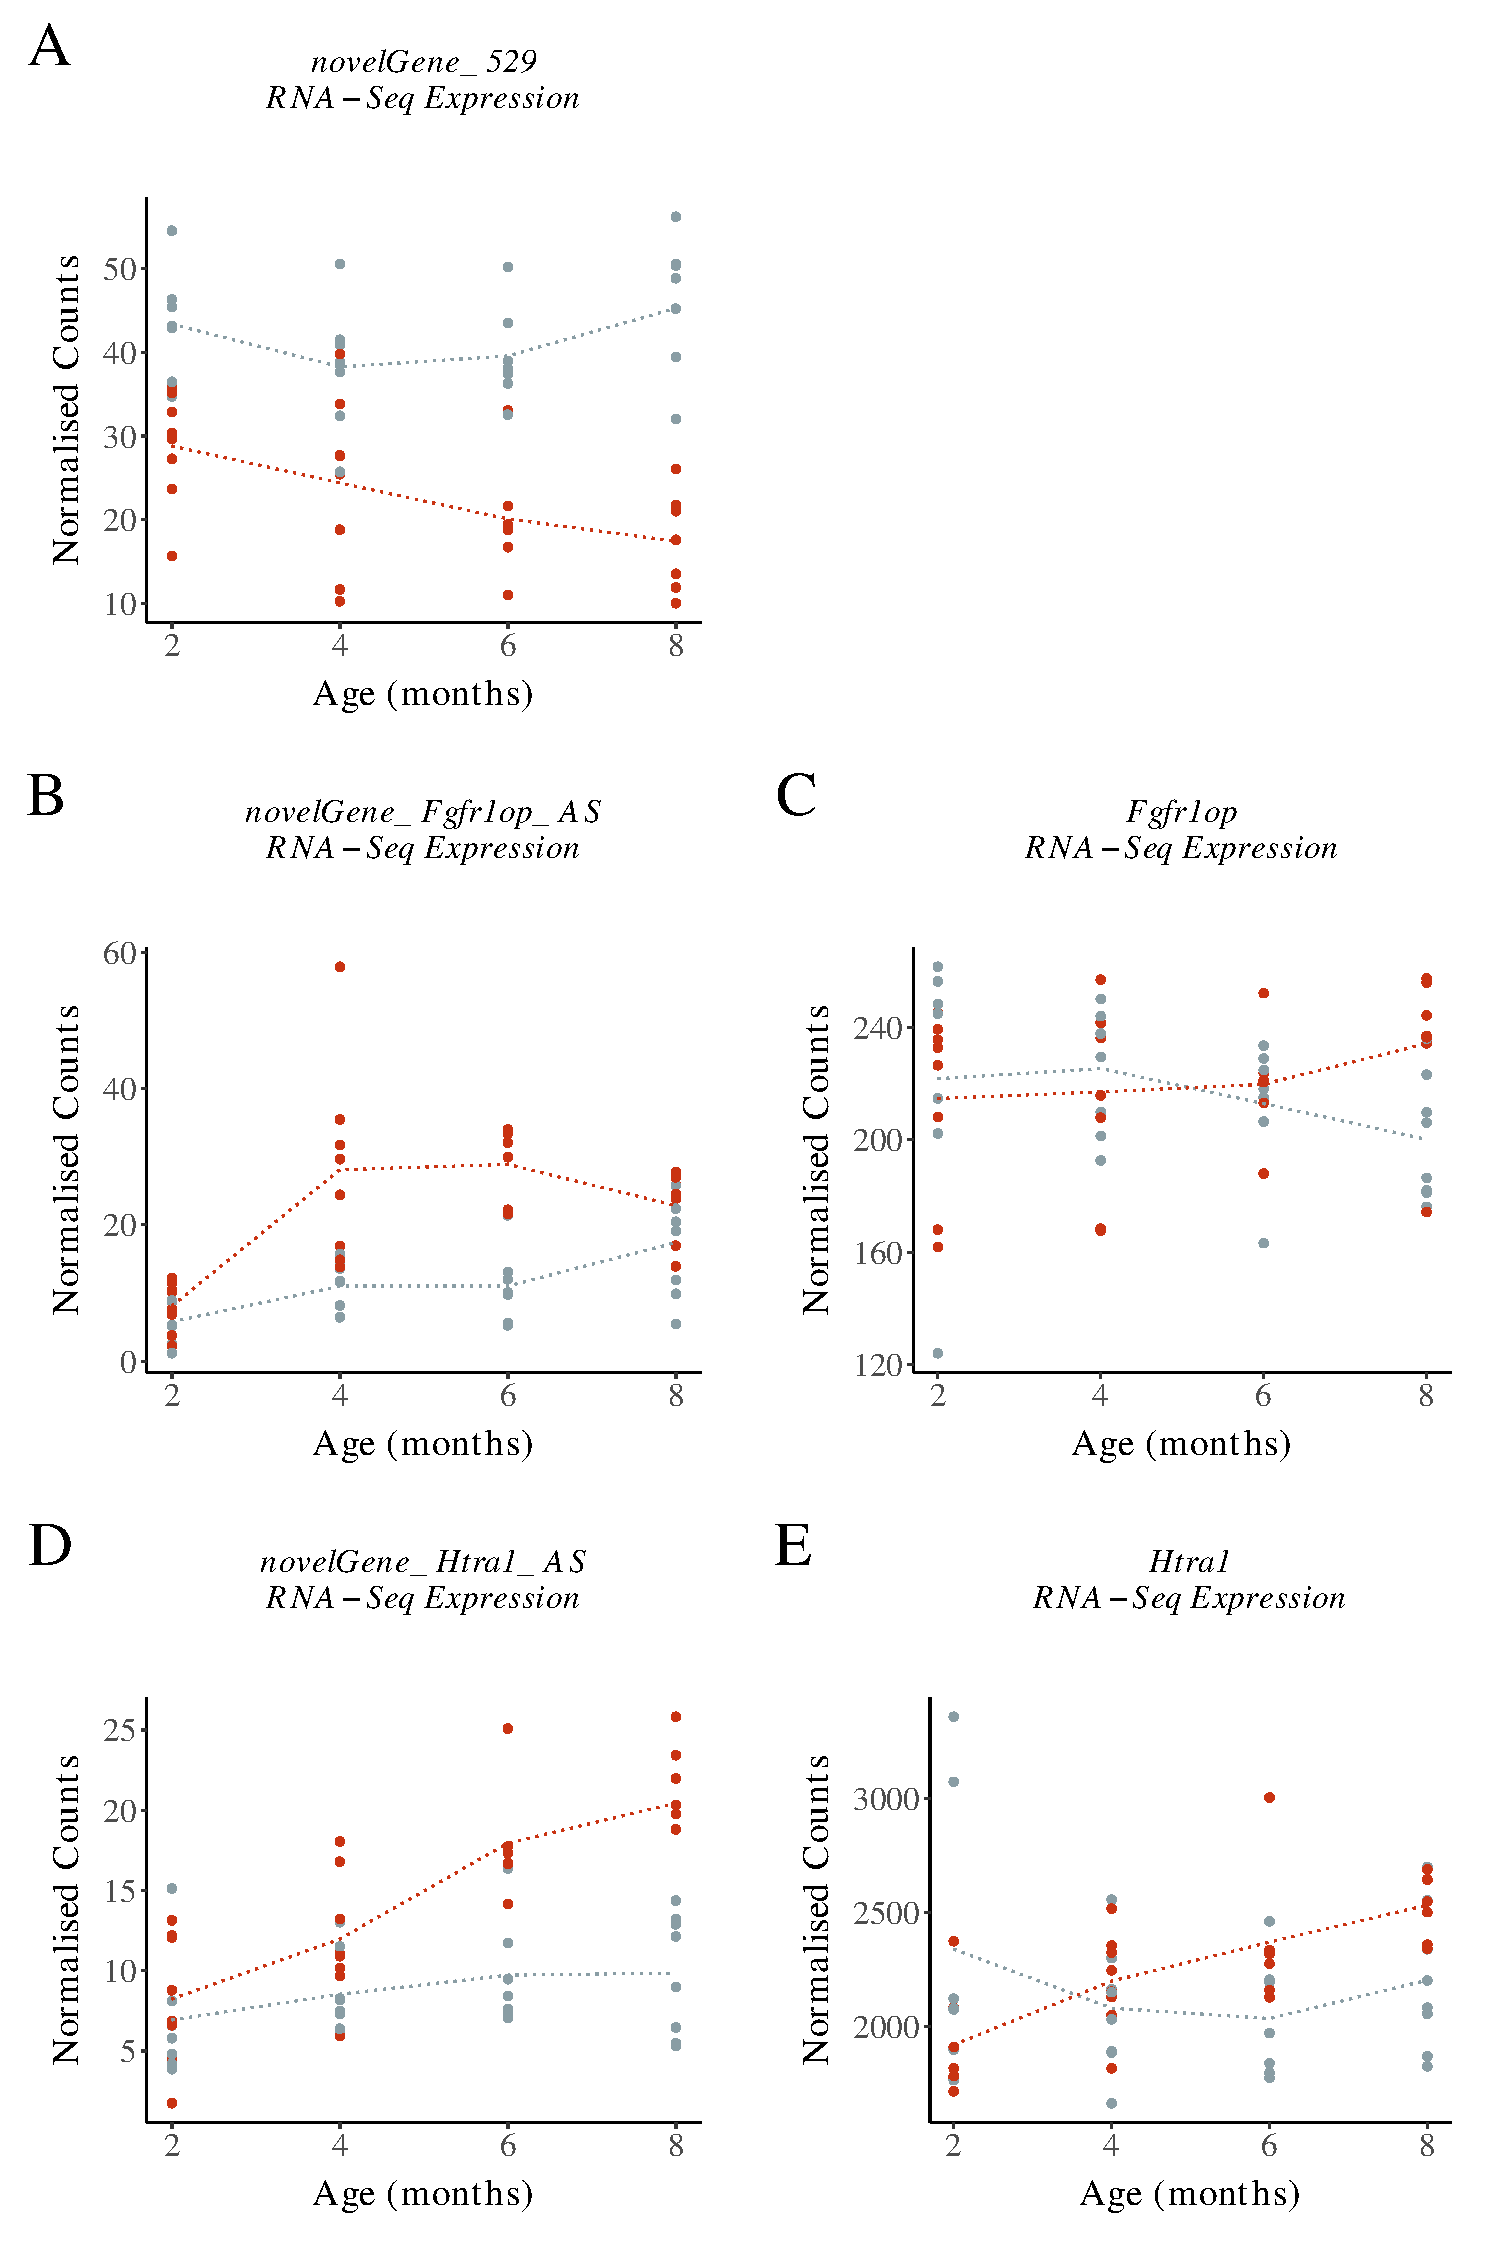
\includegraphics[page=1,scale = 0.55]{Figures/NovelGeneExp.pdf}
	\end{center}
	\captionsetup{width=0.95\textwidth}
	\caption[Three novel genes were found differentially expressed in rTg4510 TG mice]%
	{\textbf{Three novel genes were found differentially expressed in rTg4510 TG mice}: Shown are gene expression of three novel genes: \textbf{(A)} intergenic in chromosome 10 (PB.1799.1, \cref{fig:whole_novelgene_difftracks}\textbf{A}), \textbf{(B)} antisense to \textit{Fgfr1op} (PB.6616.1, \cref{fig:whole_novelgene_difftracks}\textbf{B}) and \textbf{(D)} to \textit{Htra1} (PB.15002.1, \cref{fig:whole_novelgene_difftracks}\textbf{C}). Gene expression for the two known genes, \textbf{(C)} \textit{Fgfr1op} and \textbf{(E)} \textit{Htra1} are also shown. Gene expression was determined from mapping RNA-Seq reads to Iso-Seq-derived annotations.}   
	\label{fig:whole_novelgene_diffexp}
\end{figure}

\clearpage
\subsection{Gene expression differences in rTg4510 mice are primarily driven by the differential expression of dominant isoform}
One of the added advantages of long read sequencing is the improved confidence to reliably identify isoforms with significant changes in expression across experimental conditions and over time. Given that we were able to reliably detect tau-associated differentially-expressed genes in rTg4510 TG mice using normalised FL long-read read counts (described in \cref{ch5: diffgeneexp}), we subsequently sought to identify differentially expressed \textit{transcripts} using the same approach. 

Using Iso-Seq reads for annotation and expression, we identified 886 differentially expressed transcripts, 601 (67.8\%) of which were associated with progressive tau pathology. There was a significant (exact bionomial test, n = 601 transcripts, P = 2.21 x 10\textsuperscript{-38}) enrichment of upregulated transcripts (n = 456 genes (75.9\%) in TG compared to WT; n = 145 (24.1\%) genes with downregulated expression in TG). Using \textit{EnrichR}, the differentially expressed transcripts were found to be highly enriched in the lysosome (GO Cellular Component: odds ratio = 3.25, adjusted p-value = 1.65 x 10\textsuperscript{-4}), in several molecular functions including protein kinase binding (odds ratio = 2.02, adjusted p-value = 0.048) and ATPase binding (odds ratio = 4.23, adjusted p-value = 0.048), and transcription of mouse macrophages (odds ratio= 1.90, adjusted p-value = 1.87 x 10\textsuperscript{-7}) as targets of TCF3 (odds ratio = 2.06, adjusted p-value = 5.29 x 10\textsuperscript{-5}) and IRF8 (odds ratio = 3.64, adjusted p-value = 7.11 x 10\textsuperscript{-4}) transcription factors.  

%hough tau-pathology associated expression changes in minor isoforms were significantly more pronounced - a reflection of the comparably higher sequencing coverage of RNA-Seq reads to Iso-Seq reads.

Two of the most significant differentially expressed transcripts associated with the progression of tau pathology (\cref{tab:DEI_trans}) were annotated to \textit{Gfap} (\cref{fig:DEI_gfap}) and \textit{C4b} (\cref{fig:DEI_c4b}), the top two most differentially-expressed genes (\cref{tab:dea_wholemouse}). Both genes were characterised by a dominant known isoform in rTg4510 mice: Gfap-201 (ENSMUST00000077902.5, PB.2972.16) (\cref{fig:DEI_gfap}\textbf{A,B}) and C4b-201 (ENSMUST00000069507.8, PB.7004.8) (\cref{fig:DEI_c4b}\textbf{A,B}). Expression of these two known isoforms was significantly higher than that of the novel isoforms, and was strongly up-regulated with progressive tau pathology (\cref{fig:DEI_gfap}\textbf{D}, \cref{fig:DEI_c4b}\textbf{D}), indicating that increased \textit{Gfap} (\cref{fig:whole_dea}\textbf{A}) and \textit{C4b} gene expression in aged rTg4510 transgenic mice was primarily driven by the upregulation of one specific isoform. This corroborates with previous studies that reported a differential increase of the human-equivalent \textit{Gfap-201} transcript in AD temporal cortex\cite{Roelofs2005}, and qPCR studies in AD mouse models that similarly showed upregulation of \textit{Gfap}-associated isoforms\cite{Kamphuis2012}. Furthermore, all the other minor novel isoforms, detected but not validated in previous studies\cite{Kamphuis2012}, were more abundant in the aged rTg4510 transgenic mice (\cref{fig:DEI_gfap}\textbf{C}, \cref{fig:DEI_c4b}\textbf{C}).

These findings were corroborated when using normalised read counts from short-read RNA-Seq mapped to the improved Iso-Seq-derived transcriptome annotation - both Gfap-201 (\cref{fig:DEI_gfap}\textbf{E}) and C4b-201 (\cref{fig:DEI_c4b}\textbf{E}) were found to be dramatically upregulated with progressive tau pathology. However, some of the minor novel isoforms annotated to \textit{Gfap} were also found to change with rTg4510 genotype with a more pronounced upregulation than Gfap-201 (PB.2972.8, PB.2972.17 \cref{fig:DEI_gfap}\textbf{E}). Visualisation of the different isoforms revealed that they are generally very similar (\cref{fig:DEI_gfap}\textbf{A}), with an almost identical internal exonic structure (e.g. PB.2972.8 and the known canonical isoform only differ by skipping of exon 3, PB.2972.17 contains an alternative splice site at exon 8). The sensitivity of RNA-Seq reads to differentiate these virtually-identical isoforms is therefore questionable given there are only a few loci that can be used for unambiguous assignment of RNA-Seq reads.  

\begin{figure}[!htp]
	\centering
	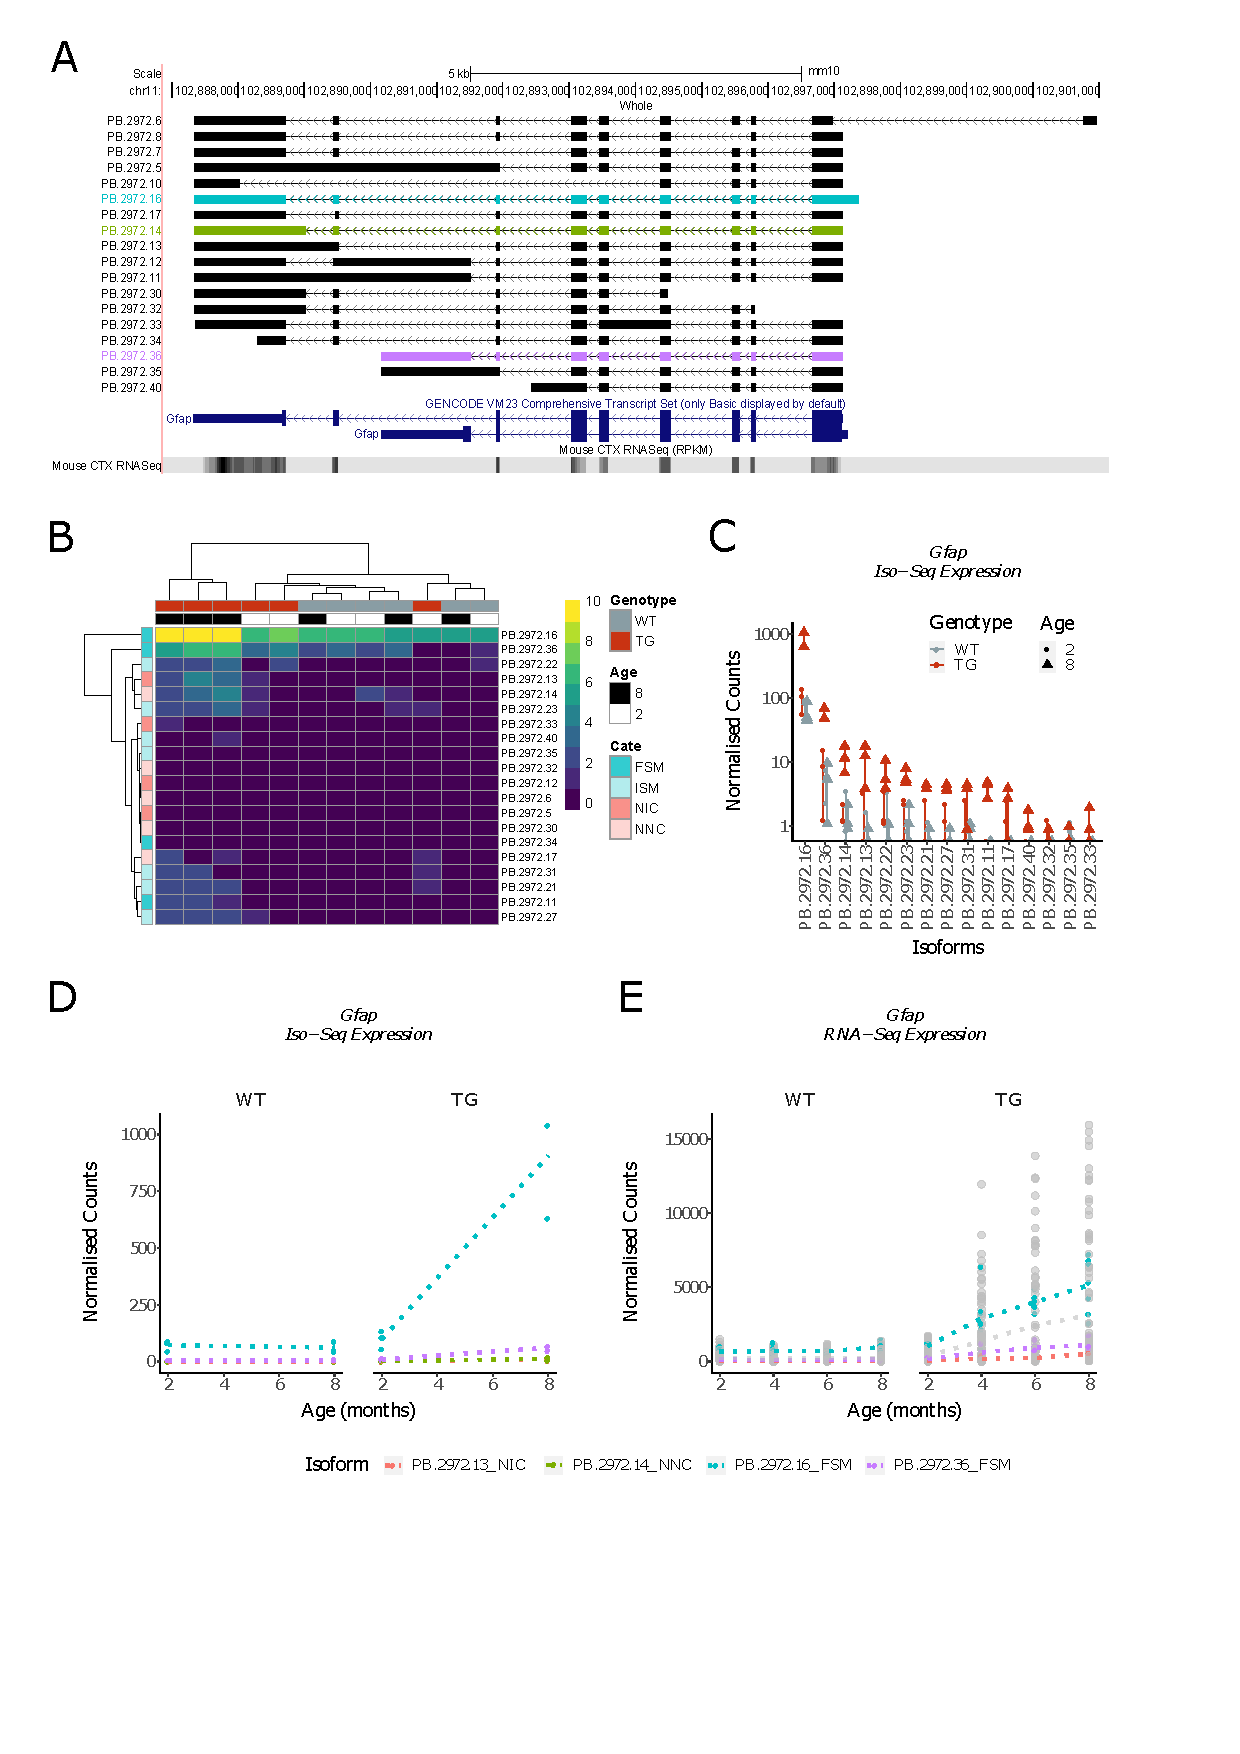
\includegraphics[page=1,trim={0.5cm 4.8cm 2cm 1cm}, scale = 0.85]{Figures/Ch5_DiffPlots.pdf}
	\captionsetup{width=0.95\textwidth}
	\caption[Differential Isoform Expression: Changes in transcript expression of isoforms associated with \textit{Gfap}]%
	{\textbf{Significant upregulation of known isoform of \textit{Gfap} with progressive tau pathology}. Shown are the \textbf{(A)} UCSC genome browser tracks of isoforms annotated to \textit{Gfap}, \textbf{(B)} hierarchal clustering of each \textit{Gfap}-associated isoform based on abundance (Iso-Seq FL read count, log2), \textbf{(C)} Normalised Iso-Seq FL read count of the top 15 most abundant isoforms, and \textbf{(D)} differentially expressed transcripts identified using normalised Iso-Seq read and \textbf{(E)} RNA-Seq read counts. Grey dots denote to differentially expressed transcripts identified from RNA-Seq but not Iso-Seq reads. FSM - Full Splice Match, ISM - Incomplete Splice Match, NIC - Novel In Catalogue, NNC - Novel Not in Catalogue. WT - Wild-type, TG - Transgenic. Dotted lines represent the mean paths across ages (months).} 
	\label{fig:DEI_gfap}
\end{figure}

\begin{figure}[!htp]
	\centering
	\includegraphics[page=2,trim={1.5cm 4.8cm 2cm 1cm}, scale = 0.85]{Figures/Ch5_DiffPlots.pdf}
	\captionsetup{width=0.95\textwidth}
	\caption[Differential Isoform Expression: Changes in transcript expression of isoforms associated with \textit{C4b}]%
	{\textbf{Significant upregulation of known isoform of \textit{C4b} with progressive tau pathology}. Shown are the \textbf{(A)} UCSC genome browser tracks of isoforms annotated to \textit{C4bp}, \textbf{(B)} hierarchal clustering of each \textit{C4b}-associated isoform based on abundance (Iso-Seq FL read count, log2), \textbf{(C)} Normalised Iso-Seq FL read count of the top 15 most abundant isoforms, and \textbf{(D)} differentially expressed transcripts identified using normalised Iso-Seq read and \textbf{(E)} RNA-Seq read counts. Grey dots denote to differentially expressed transcripts identified from RNA-Seq but not Iso-Seq reads. FSM - Full Splice Match, ISM - Incomplete Splice Match, NIC - Novel In Catalogue, NNC - Novel Not in Catalogue. WT - Wild-type, TG - Transgenic. Dotted lines represent the mean paths across ages (months).}   
	\label{fig:DEI_c4b}
\end{figure}

\clearpage
\subsection{rTg4510 mice are characterised by the differential expression of transcripts of genes implicated in AD}
\label{ch5: diffisoexp}
The list of transcripts progressively altered in rTg4510 transgenic mice included genes previously implicated in AD pathology and development (\cref{tab:DEI_trans}). This included: i) Padi2-201 (ENSMUST00000030765.6) annotated to \textit{Padi2}/\textit{Pad2} (\cref{fig:Padi2}), which encodes for an enzyme that is abnormally activated in astrocytes of AD patients \cite{A2005}, ii) H2-D1-202 (ENSMUST00000172785.7) annotated to \textit{H2-D1} (\cref{fig:H2D1}), which encodes for major histocompatibility complex (MHC) class 1, an immune-related gene that is upregulated in microglia of a neurodegenerative mouse model with AD-like phenotypes\cite{Mathys2017}, iii) Gatm-201 (ENSMUST00000028624.8) annotated to \textit{Gatm} (\cref{fig:Gatm}), encoding a mitochondrial protein recently revealed as a key AD protein signature of AD \cite{Wang2020}, and iv) Ctsd-202 (ENSMUST00000151120.8) annotated to \textit{Ctsd} (\cref{fig:Ctsd}), encoding Cathepsin D, a lysosomal protease involved in A$\beta$ \cite{JR1996} and tau \cite{A1997} degradation, and a key regulator of A$\beta$42/40 ratio\cite{Suire2020}, among others. Similarly to \textit{Gfap} and \textit{C4b}, these genes were characterised by a dominant known isoform that was significantly upregulated with progressive tau pathology, which was confirmed using RNA-Seq reads mapped to our novel transcriptome annotation. 


\begin{landscape}
\begin{table}[]
	\centering
	\captionsetup{width=1.45\textwidth}
	\caption[Differentially expressed transcripts associated with rTg4510 genotype]%
	{Tabulated are the top-ranked transcripts identified as differentially expressed in rTg4510 transgenic mice using \textit{maSigPro} with Iso-Seq defined transcriptome for annotation and Iso-Seq FL read count as expression. Rank denotes to the order of differentially expressed transcripts (n = 886) by FDR. FDR - False Discovery Rate, Mos - Months, TG - Transgenic, WT - Wild-type. }
	\begin{tabular}{@{}cccccccccc@{}}
		\toprule
		\multirow{2}{*}{Rank} &
		\multirow{2}{*}{Gene} &
		\multirow{2}{*}{Isoform} &
		\multirow{2}{*}{Isoform Id} &
		\multirow{2}{*}{FDR} &
		\multirow{2}{*}{\begin{tabular}[c]{@{}c@{}}log2-fold \\ change \\ (8 mos)\end{tabular}} &
		\multicolumn{2}{c}{\begin{tabular}[c]{@{}c@{}}Mean WT \\ Transcript expression\end{tabular}} &
		\multicolumn{2}{c}{\begin{tabular}[c]{@{}c@{}}Mean TG\\  Transcript expression\end{tabular}} \\ \cmidrule(l){7-10} 
		&                 &                       &            &            &       & 2 mos & 8 mos & 2 mos & 8 mos \\ \midrule
		1   & \textit{Ubqln1} & ENSMUST00000058735.11 & PB.4255.13 & 7.43E-42   & 0.96  & 0.969 & 33.9  & 43.4  & 22.8  \\
		2   & \textit{C4b}    & ENSMUST00000069507.8  & PB.7004.8  & 5.9E-40    & 0.942 & 4.41  & 3.49  & 1.78  & 3.86  \\
		3   & \textit{Gfap}   & ENSMUST00000077902.5  & PB.2972.16 & 1.11E-35   & 0.933 & 3.19  & 72.3  & 60.9  & 99    \\
		4   & \textit{Tgfbr1} & ENSMUST00000007757.14 & PB.10959.1 & 1.09E-19   & 0.841 & 3.16  & 0.66  & 1.31  & 1.21  \\
		5   & \textit{Cd34}   & ENSMUST00000016638.7  & PB.1036.2  & 8.43E-18   & 0.894 & 1.99  & 1.31  & 5.4   & 2.71  \\
		29  & \textit{Padi2}  & ENSMUST00000030765.6  & PB.11607.2 & 5.2E-11    & 0.792 & 2.13  & 22.6  & 24.3  & 26.7  \\
		76  & \textit{H2-D1}  & ENSMUST00000172785.7  & PB.7039.1  & 8.47E-08   & 0.697 & 1.5   & 30.6  & 28.1  & 40.3  \\
		79  & \textit{Gatm}   & ENSMUST00000028624.8  & PB.9298.1  & 9.79E-08   & 0.738 & 0.869 & 29.1  & 34.5  & 34.6  \\
		175 & \textit{Ctsd}   & ENSMUST00000151120.8  & PB.15108.6 & 0.00000592 & 0.598 & 1.03  & 89.7  & 91.8  & 127   \\ \bottomrule
	\end{tabular}
	\label{tab:DEI_trans}
\end{table}
\end{landscape}

\begin{landscape}
	\begin{figure}[!htp]
		\centering
		\includegraphics[page=4,trim={1.5cm 3.5cm 2cm 1cm}, scale = 0.85]{Figures/Ch5_DiffPlots_Landscape.pdf}
		\captionsetup{width=1.5\textwidth}
		\caption[Differential Isoform Expression: \textit{Padi2}]%
		{\textbf{Significant upregulation of \textit{Padi2-201} with progressive tau pathology}. Shown are the \textbf{(A)} UCSC genome browser tracks of isoforms annotated to \textit{Padi2}, \textbf{(B)} hierarchal clustering of each \textit{Padi2}-associated isoform based on abundance (Iso-Seq FL read count, log2), \textbf{(C)} differentially expressed transcript (Padi2-201, ENSMUST00000030765.6, PB.11607.2) identified using normalised Iso-Seq read and \textbf{(E)} RNA-Seq read counts. Grey dots denote to differentially expressed transcripts identified from RNA-Seq but not Iso-Seq reads. Dotted lines represent the mean paths across ages (months).}   
		\label{fig:Padi2}
	\end{figure}	
\end{landscape}

\begin{landscape}
	\begin{figure}[!htp]
		\centering
		\includegraphics[page=2,trim={1.5cm 3.5cm 2cm 1cm}, scale = 0.85]{Figures/Ch5_DiffPlots_Landscape.pdf}
		\captionsetup{width=1.5\textwidth}
		\caption[Differential Isoform Expression: \textit{H2-D1}]%
		{\textbf{Significant upregulation of \textit{H2-D1-202} with progressive tau pathology}. Shown are the \textbf{(A)} UCSC genome browser tracks of isoforms annotated to \textit{H2-D1}, \textbf{(B)} hierarchal clustering of each \textit{H2-D1}-associated isoform based on abundance (Iso-Seq FL read count, log2), \textbf{(C)} differentially expressed transcript (H2-D1-202, ENSMUST00000172785.7, PB.7039.1) identified using normalised Iso-Seq read and \textbf{(E)} RNA-Seq read counts. Grey dots denote to differentially expressed transcripts identified from RNA-Seq but not Iso-Seq reads. Dotted lines represent the mean paths across ages (months).}   
		\label{fig:H2D1}
	\end{figure}	
\end{landscape}

\begin{landscape}
	\begin{figure}[!htp]
		\centering
		\includegraphics[page=3,trim={1.5cm 3.5cm 2cm 1cm}, scale = 0.85]{Figures/Ch5_DiffPlots_Landscape.pdf}
		\captionsetup{width=1.5\textwidth}
		\caption[Differential Isoform Expression: \textit{Gatm}]%
		{\textbf{Significant upregulation of \textit{Gatm-201} with progressive tau pathology}. Shown are the \textbf{(A)} UCSC genome browser tracks of isoforms annotated to \textit{Gatm}, \textbf{(B)} hierarchal clustering of each \textit{Gatm}-associated isoform based on abundance (Iso-Seq FL read count, log2), \textbf{(C)} differentially expressed transcript (Gatm-201, ENSMUST00000028624.8, PB.9298.1) identified using normalised Iso-Seq read and \textbf{(E)} RNA-Seq read counts. Grey dots denote to differentially expressed transcripts identified from RNA-Seq but not Iso-Seq reads. Dotted lines represent the mean paths across ages (months).}   
		\label{fig:Gatm}
	\end{figure}	
\end{landscape}

\begin{landscape}
	\begin{figure}[!htp]
		\centering
		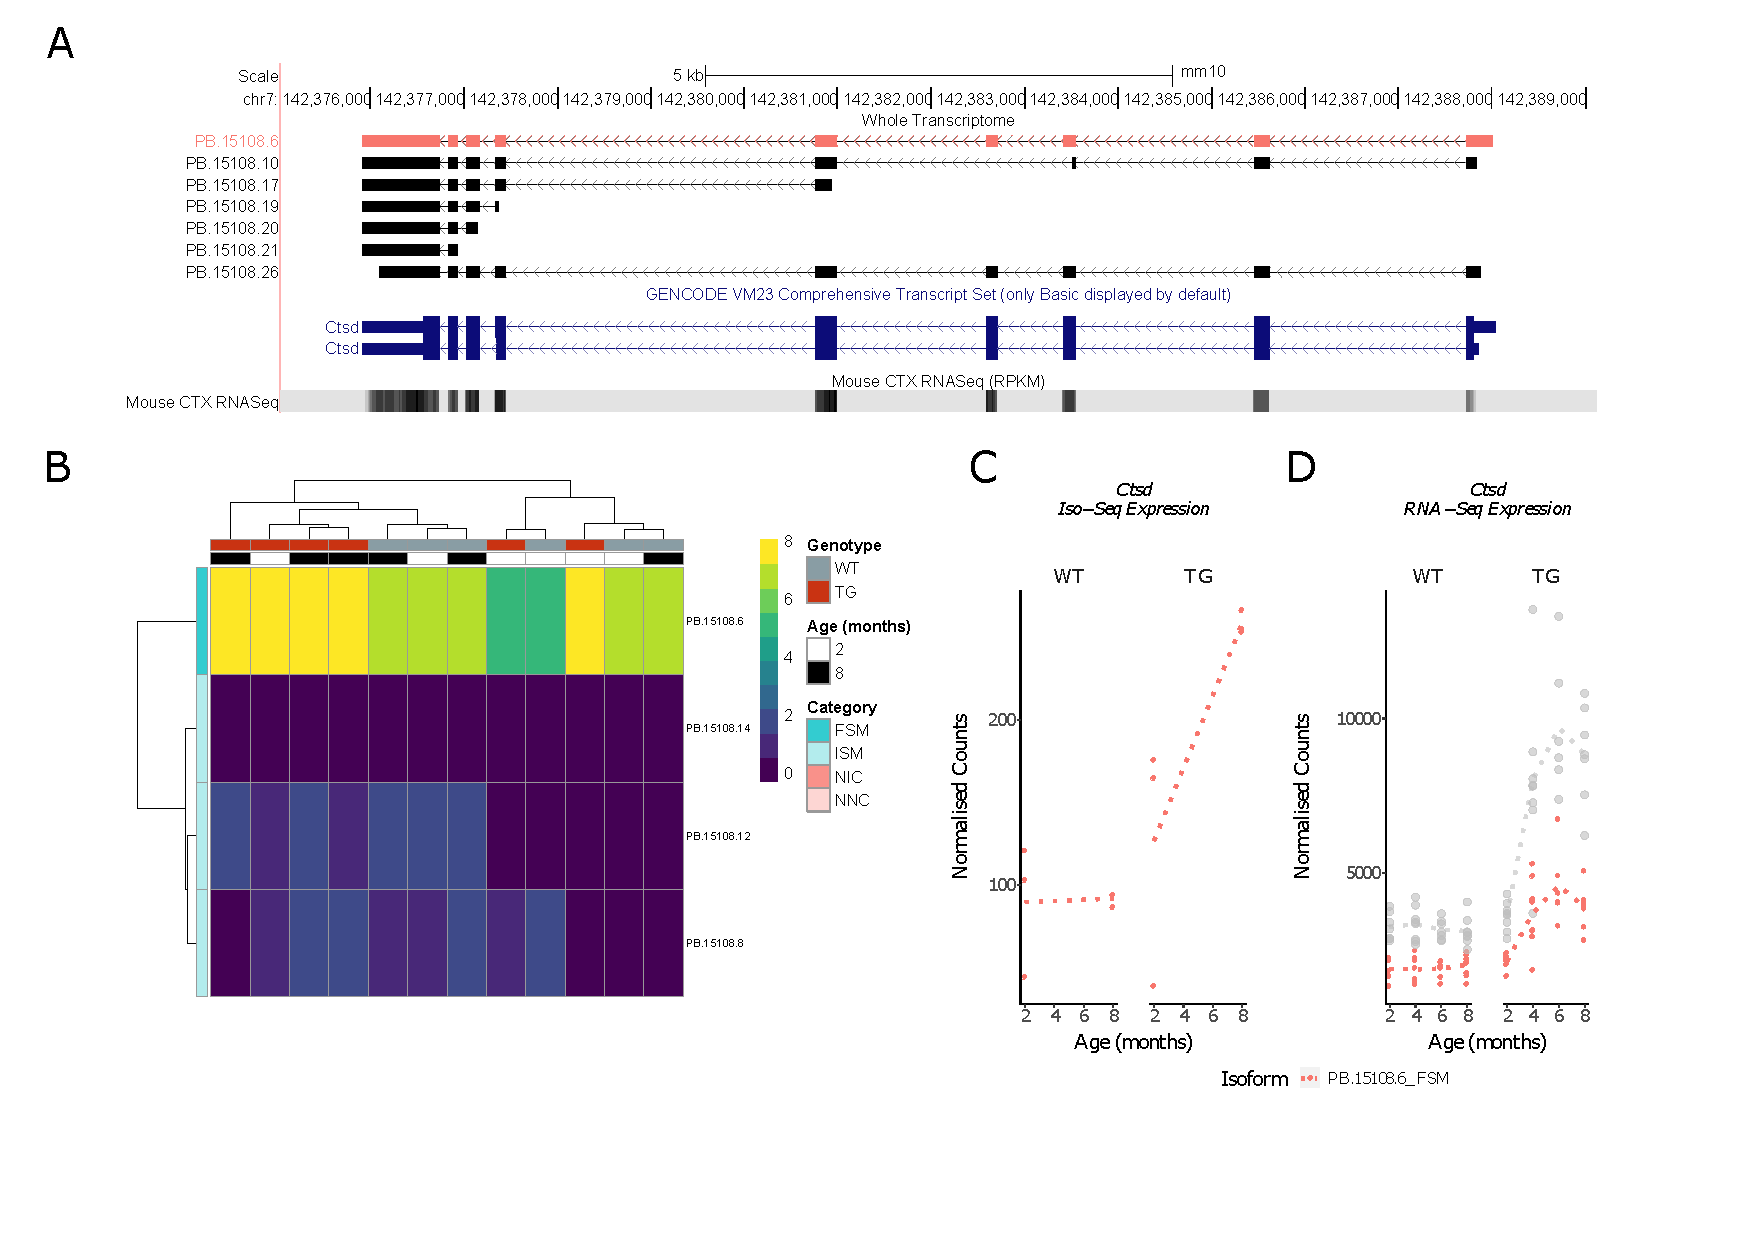
\includegraphics[page=1,trim={1.5cm 2.5cm 2cm 2cm}, scale = 0.85]{Figures/Ch5_DiffPlots_Landscape.pdf}
		\captionsetup{width=1.5\textwidth}
		\caption[Differential Isoform Expression: \textit{Ctsd}]%
		{\textbf{Significant upregulation of \textit{Ctsd-202} with progressive tau pathology}. Shown are the \textbf{(A)} UCSC genome browser tracks of isoforms annotated to \textit{Ctsd}, \textbf{(B)} hierarchal clustering of each \textit{Ctsd}-associated isoform based on abundance (Iso-Seq FL read count, log2), \textbf{(C)} differentially expressed transcript (Ctsd-202, ENSMUST00000151120.8, PB.15108.6) identified using normalised Iso-Seq read and \textbf{(E)} RNA-Seq read counts. Grey dots denote to differentially expressed transcripts identified from RNA-Seq but not Iso-Seq reads. Dotted lines represent the mean paths across ages (months).}   
		\label{fig:Ctsd}
	\end{figure}	
\end{landscape}

Despite the demonstrated utility of using long reads for differential expression analysis, we found that the expression changes for the majority of differentially-expressed transcripts identified using normalised Iso-Seq read counts (n = 545, 90.6\%) were not recapitulated with normalised RNA-Seq read counts. This included the top ranked transcript, Ubqln1-201 (ENSMUST00000058735.11, PB.4255.13) annotated to \textit{Ubqln1} and Cd34-201 (ENSMUST00000016638.7, PB.1036.2) annotated to \textit{Cd34} (\cref{tab:DEI_trans}). Although both transcripts were upregulated with progressive tau pathology in rTg4510 mice using Iso-Seq FL read counts, no significant transcript expression change was identified with normalised RNA-Seq read counts. Deeper examination of the Iso-Seq expression profiles revealed that while a change in mean expression was observed, there was a large variance. In contrast, the change in mean RNA-Seq expression was negligible due to more samples (RNA-Seq: n = 6 replicates; Iso-Seq: n = 3 replicates) and time points (RNA-Seq: 4 ages at 2, 4, 6 and 8 months; Iso-Seq: 2 ages at 2 and 8 months). We further noted that the majority of Iso-Seq-identified differentially expressed transcripts (n = 497 transcripts, 82.1\% ) were very-lowly expressed (< 24 mean normalised FL reads, n = 12 samples). 

\begin{figure}[!htp]
	\centering
	\includegraphics[page=3,trim={1.5cm 3cm 2cm 1cm}, scale = 0.80]{Figures/Ch5_DiffPlots.pdf}
	\captionsetup{width=0.95\textwidth}
	\caption[Disparities in differential transcript expression analysis]%
	{\textbf{Disparities in differential transcript expression analysis}. Shown are the \textbf{(A)} UCSC genome browser tracks of the isoforms annotated to \textit{Ubqln1}, with two isoforms identified as differentially expressed using \textbf{(B)} normalised Iso-Seq read counts but not \textbf{(C)} RNA-Seq read counts. Similarly, \textbf{(D)} USCS genome browser track of \textit{Cd34}, \textbf{(E)} Iso-Seq transcript expression profile and \textbf{(F)} RNA-Seq transcript expression profile are shown. The differentially expressed transcript identified from normalised Iso-Seq FL read counts is coloured respectively. 
	}   
	\label{fig:DEI_cd34_ubq}
\end{figure}

\clearpage
\subsection{Hybrid approach identifies tau-pathology associated differential isoform usage with major isoform switching events}
Further complexity in transcriptional regulation is reflected in the fact that the expression of a gene may remain constant between conditions, but the \textit{relative} expression of individual isoforms (and thus isoform \textit{proportions}) may differ; this phenomenon is known as differential transcript usage (DTU) and is described in detail in \cref{intro:dtu}. I therefore assessed whether the relative abundance of isoforms for each gene was associated with rTg4510 genotype and/or age, and whether there was switching of the dominant major (highest expressed) isoform between groups. 

Using Iso-Seq reads, we were not able to identify genes with differential transcript usage, likely reflecting the relatively low sequencing coverage and small sample size of our Iso-Seq experiments. In contrast, we identified 671 DTU genes (\cref{tab:DIU_DEA_nums}) when using normalised RNA-Seq read count aligned to our novel Iso-Seq-derived transcriptome (using the hybrid approach described in \cref{sec: gene_isoform_quant_explained}). Strikingly, the majority of these genes (n = 519, 77.3\%), while characterised with a change in isoform proportions, were not differentially expressed at the gene level between wild-type and transgenic mice. We further identified 61 genes that were not differentially expressed but were identified with both DTU and Major Isoform Switching, indicating that a significant degree of the post-transcriptional regulation was independent of gene expression regulation. These genes (n = 580) were enriched for targets of a number of transcription factors, particularly TAF1 (odds ratio = 1.77, adjusted p-value = 1.10 x 10\textsuperscript{-6}) - a key component of the pre-initiation complex that initiates transcription by RNA polymerase II\cite{Bieniossek2013}. 

\vspace{0.5cm}
\begin{table}[!htp]
	\centering
	\caption[Number of genes identified with differential gene expression and isoform usage]%
	{\textbf{Number of genes identified with differential gene expression and isoform usage}. Tabulated are the number of genes that are differentially expressed, and characterised with differential isoform usage and major isoform switching. Expression was determined using normalised RNA-Seq counts after alignment to Iso-Seq-defined transcriptome.}
	\begin{tabularx}{0.85\textwidth}{cccc}
		\toprule
		\multicolumn{3}{c}{Conditions}                                                                                                                                                                                       & \multirow{2}{*}{Number of Genes} \\ \cmidrule(r){1-3}
		\begin{tabular}[c]{@{}c@{}}Differential Gene\\  Expression\end{tabular} & \begin{tabular}[c]{@{}c@{}}Differential Isoform \\ Usage\end{tabular} & \begin{tabular}[c]{@{}c@{}}Major Isoform\\  Switching\end{tabular} &                                  \\ \midrule
		\checkmark  & \checkmark          & \checkmark                                                                & 16                               \\
		\checkmark                                                                      & \checkmark                                                                    & x                                                                  & 75                               \\
		x                                                                       & \checkmark                                                                    & \checkmark                                                                 & 61                               \\
		x                                                                       & \checkmark                                                                    & x                                                                  & 519                              \\ \midrule
		\multicolumn{3}{c}{Total Number of Genes}                                                                                                                                                                            & 671                              \\ \bottomrule
	\end{tabularx}
	\label{tab:DIU_DEA_nums}
\end{table}

The top gene characterised by a major isoform switch was \textit{Cisd3} (FDR = 3.26 x 10\textsuperscript{-26}, \cref{fig:DIU_Cisd3}\textbf{A}), a mitochondrial iron-sulphur domain-containing protein involved in regulating iron homeostasis essential for normal mitochondrial function\cite{Wiley2007}. While there was little change in overall gene expression (\cref{fig:DIU_Cisd3}\textbf{B}), a major isoform shift was observed between rTg4510 genotype that was consistent across all ages (\cref{fig:DIU_Cisd3}\textbf{C-E}). The two known isoforms only differed at the 5'end by an intron retention event occurring between exons 1 and 2, generating a shortened open reading frame that could potentially translate to a different N-terminal peptide sequence for the protein (\cref{fig:DIU_Cisd3}\textbf{A}). Cisd3-201 (ENSMUST00000107583.2, PB.2833.2), which contains the intron retention event, was upregulated with progressive tau pathology, while Cisd3-202 (ENSMUST00000107584.7, PB.2833.1) was downregulated.  

Another gene with significant DIU but no change in gene expression was \textit{Shisa5} (FDR = 1.26 x 10\textsuperscript{-11}, \cref{fig:DIU_shisa5}\textbf{A}), a transmembrane that modulate both WNT and FGF signalling by inhibiting their maturation and trafficking to the cell surface\cite{Yamamoto2005}. A perfect example of the compensatory mechanism with differential transcript expression, we identified a gradual isoform shift associated with progressive tau pathology (\cref{fig:DIU_shisa5}\textbf{D,E}). The two isoforms of interest differed significantly in length due to usage of an alternative promoter (\cref{fig:DIU_shisa5}\textbf{A}); the longer isoform (Shisa5-201, ENSMUST00000026737.11, PB.16934.2) spanned the full-length of the gene across all 6 exons, whereas the shorter isoform (Shisa5-203, ENSMUST00000154184.4, PB.16934.9) lacked the first 3 upstream exon but contained an alternative first exon. Unsurprisingly, ORF prediction revealed a significant disparity in the reading frame length with the longer isoform containing the whole Shisa Pfam domain. While the shorter isoform was the dominant isoform in wild-type across all ages, we observed a downregulation of this isoform coupled with a drastic upregulation of the longer transcript in rTg4510 transgenic mice (\cref{fig:DIU_shisa5}\textbf{C,D}), resulting in zero net change in gene expression (\cref{fig:DIU_shisa5}\textbf{B}). 

In addition to identifying genes with DIU without differential gene expression, we also identified genes with evidence for altered gene expression accompanied with differential isoform expression and major isoform switching. This included \textit{Fblim1} (FDR = 1.87 x 10\textsuperscript{-13}, \cref{fig:DIU_fblim1}\textbf{A}) - a gene that encodes for a filamin-binding protein that is involved in actin filament assembly and plays a role in cell adhesion\cite{Takafuta2003} - which was upregulated with progressive tau pathology in rTg4510 transgenic mice. Drawing parallels to \textit{Gfap} and \textit{C4b}, increased \textit{Fblim1} gene expression was also primarily driven by one isoform (\cref{fig:DIU_fblim1}\textbf{B}). However, this isoform was the less abundant, minor known isoform, Fblim1-203 (ENSMUST00000105785.8, PB.11626.1) found in wild-type mice rather than the dominant known isoform, Fblim1-202 (ENSMUST00000105784.7, PB.11626.2) (\cref{fig:DIU_fblim1}\textbf{D,E}). Given that detection of Fblim1-203 was negligible in wild-type mice, drastic upregulation of this isoform associated with progressive tau pathology resulted in a robust isoform switch (\cref{fig:DIU_fblim1}\textbf{C}). Characterisation of these two isoforms revealed that they only differed by the presence of an alternative first exon, with the reading frame being broadly similar (\cref{fig:DIU_fblim1}\textbf{A}). 

Finally, we identified a novel fusion gene, \textit{Arpc4-Ttll3} (the phenomenon of fusion genes is described in \cref{ch4:fusion_trans}) that was characterised by altered transcript usage and major isoform switching (FDR = 1.28 x 10\textsuperscript{-4}). Not existing in the reference genome, three read-through transcripts (PB.13540.3, PB.13540.7, PB.13540.8) were annotated across the full length of \textit{Arpc4}, which encodes one of the subunits of the Arp2/3 protein complex involved in actin polymerisation, and \textit{Ttll3}, which encodes the tubulin tyrosine ligase-like 1 (\cref{fig:DIU_Arpc4}\textbf{A}). The three transcripts differed by only 45bp at the first exon and the presence of exon 13 (exon 8 in \textit{Ttll3}) in PB.13540.7, which was skipped in the other two isoforms (\cref{fig:DIU_Arpc4}\textbf{A}). While there was no change in overall gene expression (\cref{fig:DIU_Arpc4}\textbf{B}), we observed an isoform switch with upregulation of PB.13540.7 and downregulation of PB.13540.3 in rTg4510 TG (\cref{fig:DIU_Arpc4}\textbf{C}), over time (\cref{fig:DIU_Arpc4}\textbf{D,E}). ORF predictions showed that skipping of exon 13 maintained the reading frame, although the predicted frame for all three transcripts only covered \textit{Ttll3} rather than across both genes (\cref{fig:DIU_Arpc4}\textbf{A}).  

\newpage
\begin{figure}[!htp]
	\centering
	\includegraphics[page=4,trim={1.5cm 3.5cm 2cm 1cm}, scale = 0.80]{Figures/Ch5_DiffPlots.pdf}
	\captionsetup{width=0.95\textwidth}
	\caption[Differential isoform expression and usage of \textit{Cisd3}]%
	{\textbf{Differential isoform expression and usage of \textit{Cisd3}}: Shown are the \textbf{(A)}  UCSC genome browser tracks of the isoforms annotated to \textit{Cisd3} with the two differentially expressed isoforms colour-coded and the respective predicted open reading frame (black), \textbf{(B)} \textit{Cisd3} gene expression, \textbf{(C)} proportion of isoform usage with rTg4510 genotype, independent of age, \textbf{(D)} \textit{Cisd3}-associated transcript expression and \textbf{(E)} proportion of isoform usage by age and genotype. Expression is determined from normalised RNA-Seq read counts after alignment to Iso-Seq-defined transcriptome.}    
	\label{fig:DIU_Cisd3}
\end{figure}

\begin{figure}[!htp]
	\centering
	\includegraphics[page=5,trim={1.5cm 1.5cm 2cm 1cm}, scale = 0.80]{Figures/Ch5_DiffPlots.pdf}
	\captionsetup{width=0.95\textwidth}
	\caption[Differential isoform expression and usage of \textit{Shisa5}]%
	{\textbf{Differential isoform expression and usage of \textit{Shisa5}}: Shown are the \textbf{(A)}  UCSC genome browser tracks of the isoforms annotated to \textit{Shisa5} with the two differentially expressed isoforms colour-coded, \textbf{(B)} \textit{Shisa5} gene expression, \textbf{(C)} proportion of isoform usage with rTg4510 genotype, independent of age, \textbf{(D)} \textit{Shisa5}-associated transcript expression and \textbf{(E)} proportion of isoform usage by age and genotype. Expression is determined from normalised RNA-Seq read counts after alignment to Iso-Seq-defined transcriptome.} 
	\label{fig:DIU_shisa5}
\end{figure}

\begin{figure}[!htp]
	\centering
	\includegraphics[page=6,trim={1.5cm 3cm 2cm 1cm}, scale = 0.80]{Figures/Ch5_DiffPlots.pdf}
	\captionsetup{width=0.95\textwidth}
	\caption[Differential isoform expression and usage of \textit{Fblim1}]%
	{\textbf{Differential isoform expression and usage of \textit{Fblim1}}: Shown are the \textbf{(A)} UCSC genome browser tracks of the isoforms annotated to \textit{Fblim1} with the two differentially expressed isoforms colour-coded and the respective predicted open reading frame (black), \textbf{(B)} \textit{Fblim1} gene expression, \textbf{(C)} proportion of isoform usage with rTg4510 genotype, independent of age, \textbf{(D)} \textit{Fblim1}-associated transcript expression and \textbf{(E)} proportion of isoform usage by age and genotype. Expression is determined from normalised RNA-Seq read counts after alignment to Iso-Seq-defined transcriptome.} 
	\label{fig:DIU_fblim1}
\end{figure}

\begin{figure}[!htp]
	\centering
	\includegraphics[page=7,trim={1.5cm 1.5cm 2cm 1cm}, scale = 0.80]{Figures/Ch5_DiffPlots.pdf}
	\captionsetup{width=0.95\textwidth}
	\caption[Differential isoform expression and usage of \textit{Arpc4-Ttll3}]%
	{\textbf{Differential isoform expression and usage of \textit{Arpc4-Ttll3}}: Shown are the \textbf{(A)} UCSC genome browser tracks of the three fusion transcripts annotated to \textit{Arpc4-Ttll3} with exon skipping (purple) and the respective predicted open reading frame (black), \textbf{(B)} \textit{Arpc4-Ttll3} gene expression, \textbf{(C)} proportion of isoform usage with rTg4510 genotype \textbf{(D)} expression of the fusion transcripts and \textbf{(E)} proportion of isoform usage by age and genotype. Expression is determined from normalised RNA-Seq read counts after alignment to Iso-Seq-defined transcriptome.} 
	\label{fig:DIU_Arpc4}
\end{figure}





\clearpage
\subsection{Integrative data analysis reveals co-localisation of genotype-associated differentially expressed transcripts and differentially-methylated positions associated with tau pathology}
Epigenetic modifications such as DNA methylation are strongly associated with gene regulation and alternative splicing. Using genome-wide DNA methylation data generated on the same mouse samples as part of another project, we subsequently sought to implement an integrative approach to identify genes with both splicing and DNA methylation differences between wild-type and transgenic mice. Genes were identified as being 'differentially spliced' if we observed a change in transcript expression (DTE), usage of isoform proportions (DTU) or both between groups. For a more consistent analysis, transcript expression was determined using normalised RNA-Seq read counts after alignment to our Iso-Seq-derived transcriptome. Differential DNA methylation, measured using Reduced Reprentation Bisulfite Sequencing (RRBS), was determined either at a specific cytosine position (differentially methylated positions - DMPs) associated with tau pathology (genotype effect) and progressively over time (interaction effect), or across broader genomic regions of differentially methylated cytosines (differentially methylated regions - DMRs). 

Focusing first on genotype-associated differentially methylated regions, we identified robust splicing changes annotated to \textit{As3mt}, a schizophrenia-associated gene that encodes for a methyltransferase (\cref{fig:IntMeth_As3mt}). In detecting three isoforms annotated to \textit{As3mt}, we observed an upregulation of the known isoform (As3mt-201, ENSMUST00000003655.8, PB.8363.2) associated with progressive tau pathology in TG mice (P = 5.92 x 10\textsuperscript{-18}, R\textsuperscript{2} = 0.57), while there was no significant expression change of the other two novel isoforms. Further examination of these isoforms revealed that both novel isoforms differed to the known isoform by an alternative first exon and the presence of a 45-97bp novel exon, located between exons 11 and 12 and supported by RNA-Seq data by matched samples. Notably, we detected an intronic 485bp DMR \textasciitilde{}8kb upstream of this novel exon, consisting of nine differentially methylated sites (hypermethylated in TG compared to WT, $\Delta$ = 0.19, P = 1.22 x 10\textsuperscript{-8}). Given the proximity of the DMR and novel exon, we hypothesise that an increase in methylation in this region could hinder recruitment and assembly of the spliceosome, resulting in skipping of the novel exon and subsequent increased expression of the known isoform. ORF predictions showed that skipping of this novel exon maintained the reading frame, whereas the reading frame of the two novel isoforms were shortened due to the presence of the novel splice site. 

In addition to \textit{As3mt}, we also identified a genotype-associated DMR and splicing change annotated to \textit{Prnp} with upregulated expression of 2 isoforms in TG mice. However, given that \textit{Mapt} transgene contains exons 2 and 3 of the mouse \textit{Prnp} gene (shown in \cref{mapt_transgene_whole}), we suspected that the transcript expression change (determined from normalised RNA-Seq read counts) was attributed to the human transgene rather than the mouse. Notably,  we did not detect differential transcript expression in \textit{Prnp} from normalised Iso-Seq read counts, further indicating that \textit{Prnp}'s altered expression and splicing change are a direct consequence of transgene activation\cite{Castanho2020}. 

\begin{figure}[htp]
	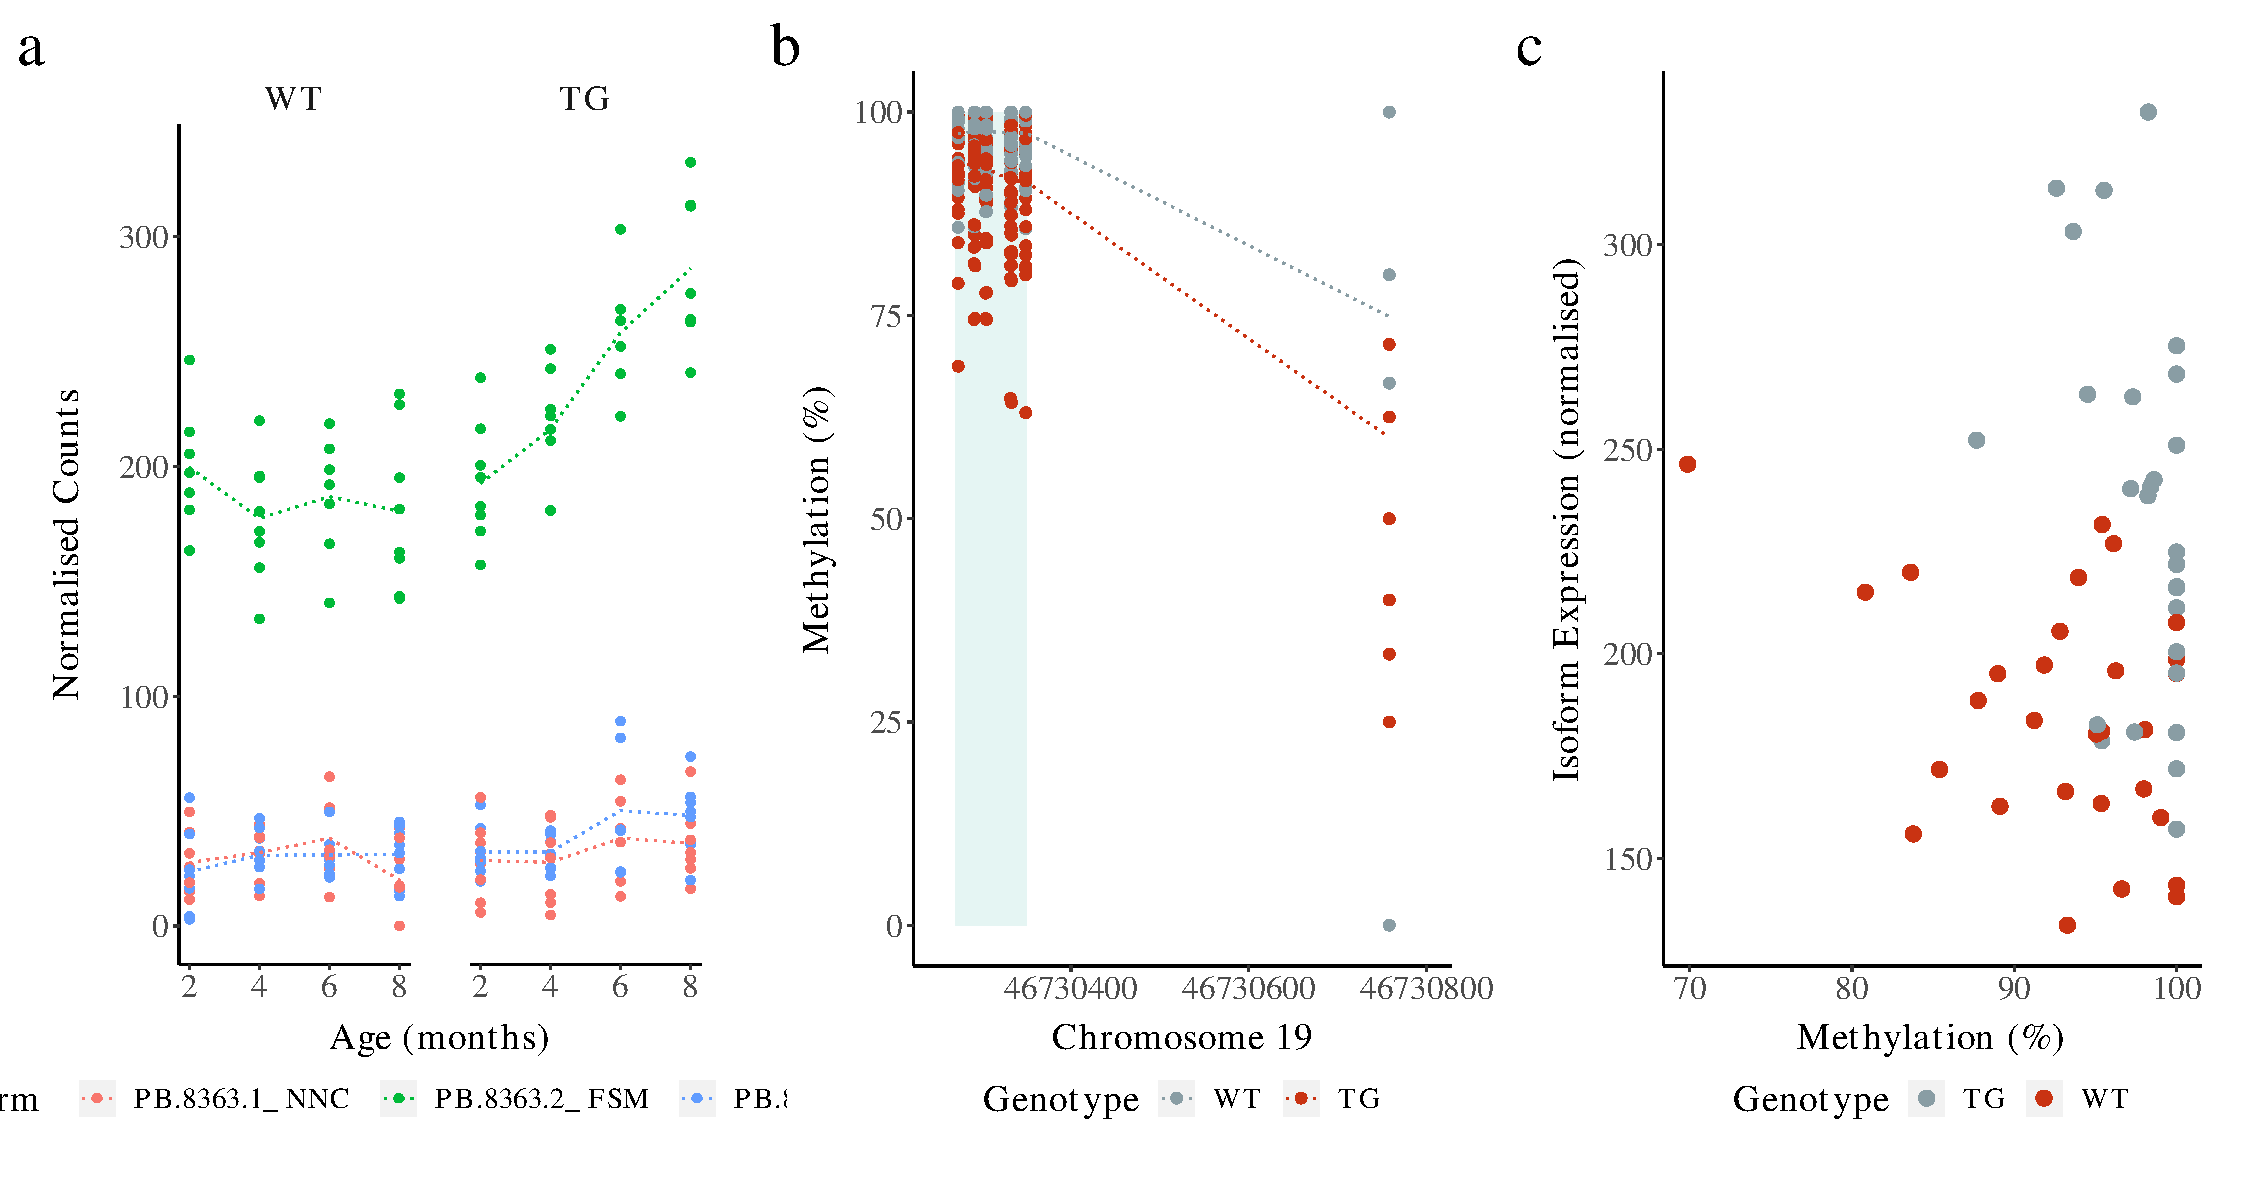
\includegraphics[page=1,scale = 0.4]{Figures/WholeDifferentialAnalysis_DMPDMR.pdf}
	\\
	\hspace*{0.2cm}\vspace{0.5cm}\large c
	\\
	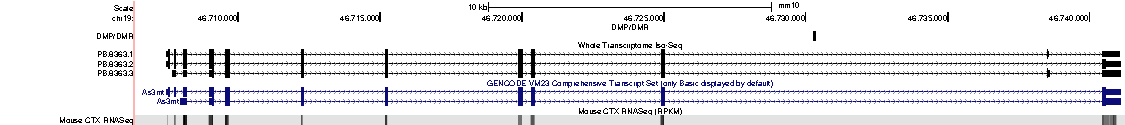
\includegraphics[page=1,trim={1.5cm 0 0 0},scale = 0.9]{Figures/AS3MT_DMP.pdf}
	\captionsetup{width=0.95\textwidth}
	\caption[Differential splicing and methylation of \textit{As3mt}]%
	{\textbf{Differential splicing and methylation of \textit{As3mt}}: \textbf{A}) Upregulation of known isoform associated with \textit{As3mt} (PB.8363.2, ENSMUST00000003655.8) in TG (P = 4.98 x 10\textsuperscript{-18}, R\textsuperscript{2} = 0.56) \textbf{(B)} A DMR of nine hypermethylated sites was identified upstream of 11th novel exon. \textbf{(D)} UCSC browser track showing relative position of DMR and isoform}    
	\label{fig:IntMeth_As3mt}
\end{figure}	

Focusing next on differentially methylated positions (DMP) associated with rTg4510 genotype and age, we identified 20 genes with a significanly altered splicing and DNA methylation profile. The vast majority of these genes were characterised with differential transcript expression (n = 18, 90\%) with significant enrichment (exact binomial test, n = 18 genes, P = 0.0308) of upregulated transcripts associated with rTg4510 genotype (n = 14, 77.8\%) in line with previous results. From these genes, the DMP location was broadly balanced between promoter (n = 5, 27.8\%), intron (n = 8, 44.4\%) and distal intergenic region (3kb upstream or downstream of the gene, n = 5, 27.8\%). Among these, there was an enrichment of hypermethylation (n = 13 genes (72.2\%) with increased methylation in TG compared to WT; n = 5 genes (27.8\%) with decreased methylation in TG).  

The top ranked gene with differential methylation and transcript expression was \textit{Osmr}, which encodes for a cytokine receptor and is a marker for reactive astrocytes. Detecting only the known isoform (Osmr-201, ENSMUST00000022746.12, PB.5258.1) which was significantly upregulated with progressive tau pathology, we identified 11 hypermethylated DMP in the promoter; increased Osmr-201 expression correlated with increased methylation in TG (corr = 0.464, p = 2.45 x 10\textsuperscript{-4}) with time (R\textsuperscript{2} = 0.77, F(6,51) = 32.19, p = 2.98 x 10\textsuperscript{-5}). Other differentially-spliced-methylated genes include: i) \textit{Ncf2} (\cref{fig:IntMeth_Ncf2}), which encodes a subunit of NAPDH oxidase that is important for phagocytosis, whereby increased expression of the known isoform (Ncf2-201, ENSMUSE00000537720.3, PB.700.1) correlated with increased methylation in TG over time (R\textsuperscript{2} = 0.81, F(6,51) = 40.23, p = 4.52 x 10\textsuperscript{-8}); ii) \textit{Irf8}, which encodes a transcription factor of the IRF family that is involved in microglial activation in AD\cite{Zeng2017}, whereby increased expression of the known isoform also correlated with increased methylation with progressive tau pathology (R\textsuperscript{2} = 0.80, F(6,34) = 27.1, p = 1.86 x 10\textsuperscript{-5}). 


Other genes were characterised with a change in transcript expression correlated with a change in DNA methylation. This included \textit{Ncf2} (\cref{fig:IntMeth_Ncf2}), \textit{Osmr}, and \textit{Cebpa} where there was a progressive increase in expression of the respective known isoform and an associated hypomethylated DMP (located in the promoter) in transgenic; whereas in \textit{Rnf165} and \textit{Susd5} (\cref{fig:IntMeth_Susd5}), there was a progressive downregulation of known isoform and an associated hypermethylated DMP in transgenic. Interestingly, we also identified altered splicing and methylation changes in \textit{Irf8} (\cref{fig:IntMeth_Irf8}) - a transcription factor of the IRF family that is involved in microglial activation in AD\cite{Zeng2017}, where a hypomethylated DMP (located 130kb downstream) in TG was associated with progressive increase in transcript expression. The associations described here between DNA methylation and transcript expression support well-established theories of the relationship between DNA methylation and gene expression, whereby increased methylation at the promoter is associated with decreased gene expression. Of note, only one isoform was detected for each of these genes.  
% Note other example where this was not the case  

This included \textit{Spata13} - a gene involved in cell migration\cite{Bourbia2019} and has been reported to be upregulated in entorhinal cortex of AD patients\cite{Yan2019} - which was characterised with a change in usage. There was a significant progressive increase in expression of the shorter known isoform (PB.4966.2, ENSMUST00000162945.1) in the transgenic mice, whereas there was no change in expression of the longer, novel NIC isoform (PB.4966.1) which harboured a 5' miRNA-binding site (miR-446h-5p) and an alternative transcription start site with an upstream open reading frame (\cref{fig:IntMeth_Spata13}\textbf{a, d}). A DMP was identified upstream of \textit{Spata13} (8.9Kb and 107Kb from known and novel isoform respectively, \cref{fig:IntMeth_Spata13}\textbf{b, d}) and was hypermethylated in transgenic mice compared to wild-type ($\Delta$$\beta$ = 0.777, FDR\textsubscript{interaction} = 0.012), \cref{fig:IntMeth_Spata13}\textbf{C}), suggesting a distal suppressed expression of both isoforms in the wild-type. Conversely, the decreased methylation in the transgenic is only associated with suppressed expression of the proximal, novel isoform. 

\begin{figure}[ht]
	\includegraphics[page=2,scale = 0.4]{Figures/WholeDifferentialAnalysis_DMPDMR.pdf}
	\\
	\hspace*{0.2cm}\vspace{0.5cm}\large d
	\\
	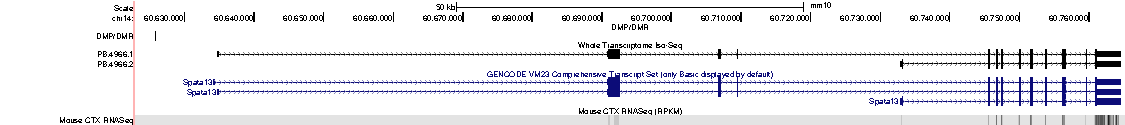
\includegraphics[page=1,trim={1.5cm 0 0 0},scale = 0.9]{Figures/SPATA13_DMP.pdf}
	\captionsetup{width=0.95\textwidth}
	\caption[Differential splicing and methylation of \textit{Spata13}]%
	{\textbf{Differential splicing and methylation of \textit{Spata13}}: \textbf{A}) Upregulation of known isoform (PB.4966.2, ENSMUST00000162945.1) associated with \textit{Spata13} in TG (P = 9.42 x 10 \textsuperscript{-33}, R\textsuperscript{2} = 0.73) \textbf{(B)} Hypermethylated DMP identified upstream of promoter ($\Delta$$\beta$ = 0.777, FDR\textsubscript{interaction} = 0.012). \textbf{(C)} Correlation between DNA methylation at this site and normalised isoform expression of the \textit{Spata13} gene. \textbf{(D)} UCSC browser track showing relative position of DMP and two isoforms. }    
	\label{fig:IntMeth_Spata13}
\end{figure}

\begin{figure}[h]
	\includegraphics[page=3,scale = 0.4]{Figures/WholeDifferentialAnalysis_DMPDMR.pdf}
	\\
	\hspace*{0.2cm}\vspace{0.5cm}\large d
	\\
	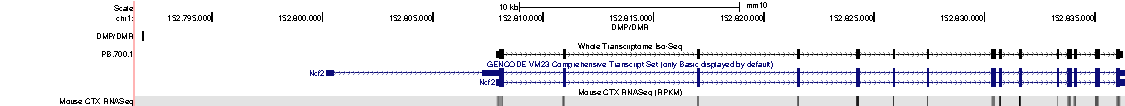
\includegraphics[page=1,trim={1.5cm 0 0 0},scale = 0.9]{Figures/NCF2_DMP.pdf}
	\captionsetup{width=0.95\textwidth}
	\caption[Differential splicing and methylation of \textit{Ncf2}]%
	{\textbf{Differential splicing and methylation of \textit{Ncf2}}. \textbf{A}) Upregulation of known isoform associated with \textit{Ncf2} (PB.700.1,ENSMUST00000027754.6) in TG coincided with two \textbf{(B)} hypomethylated DMP located upstream of promoter. Only the most significant DMP is shown ($\Delta$$\beta$ = -0.293, FDR\textsubscript{interaction} = 0.039). \textbf{(C)} Correlation between DNA methylation at this site and normalised isoform expression of the \textit{Ncf2} gene. \textbf{(D)} UCSC browser track showing relative position of DMP and isoform.}    
	\label{fig:IntMeth_Ncf2}
\end{figure}

\begin{figure}[]
	\includegraphics[page=4,scale = 0.4]{Figures/WholeDifferentialAnalysis_DMPDMR.pdf}
	\\
	\hspace*{0.2cm}\vspace{0.5cm}\large d
	\\
	
\includegraphics[page=1,trim={1.5cm 0 0 0},scale = 0.9]{Figures/SUSD5_DMP.pdf}
	\captionsetup{width=0.95\textwidth}
	\caption[Differential splicing and methylation of \textit{Susd5}]%
	{\textbf{Differential splicing and methylation of \textit{Susd5}}: \textbf{A}) Downregulation of known isoform associated with \textit{Susd5} (PB.16983.1,ENSMUST00000135338.2) in TG (P = 5.93 x 10\textsuperscript{-52}, R\textsuperscript{2} = 0.84) \textbf{(B)} Five hypermethylated DMPs were identified in the intronic region after the first exon. Only the most significant DMP is shown ($\Delta$$\beta$ = 0.344, P\textsubscript{Genotype} = 1.63). \textbf{(C)} Correlation between DNA methylation at this site and normalised isoform expression of the \textit{Susd5} gene. \textbf{(D)} UCSC browser track showing relative position of DMPs and isoform}    
	\label{fig:IntMeth_Susd5}
\end{figure}

\begin{figure}[]
	\includegraphics[page=5,scale = 0.4]{Figures/WholeDifferentialAnalysis_DMPDMR.pdf}
	\\
	\hspace*{0.2cm}\vspace{0.5cm}\large d
	\\
	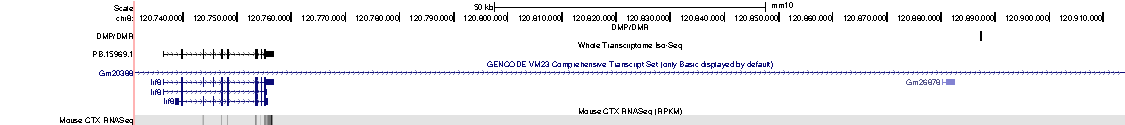
\includegraphics[page=1,trim={1.5cm 0 0 0},scale = 0.9]{Figures/IRF8_DMP.pdf}
	\captionsetup{width=0.95\textwidth}
	\caption[Differential splicing and methylation of \textit{Irf8}]%
	{\textbf{Differential splicing and methylation of \textit{Irf8}}: \textbf{A}) Upregulation of known isoform associated with \textit{Irf8} (PB.15969.1, ENSMUST00000047737.9) in TG (P = 8.17 x 10\textsuperscript{-78}, R\textsuperscript{2} = 0.87)\textbf{B)} Two hypermethylated DMPs were identified downstream in the distal intergenic region. Only the most significant DMP is shown ($\Delta$$\beta$ = -0.464, FDR\textsubscript{Interaction} = 0.0368) \textbf{(C)} Correlation between DNA methylation at this site and normalised isoform expression of the \textit{Irf8} gene. \textbf{(D)} UCSC browser track showing relative position of DMPs and isoform}    
	\label{fig:IntMeth_Irf8}
\end{figure}



\clearpage
\section{Discussion}

\subsection{Overview of results}
\begin{enumerate}
	\item First extensive study to examine differential isoform analysis on mouse model of AD pathology using long-read sequencing with 3 replicates at 2 ages 
	\item Identified widespread gene expression changes paralleling development of tau pathology in rTg4510 mice using normalised Iso-Seq FL read counts alone, demonstrating that our study was well powered to identify gene expression differences (Gfap, C4b) using long reads alone without RNA-Seq
	\item Demonstrating the utility of long reads for isoform expression analysis, further identified robust genotype-associated differences in transcripts annotated to genes implicated in AD with examples of a dominant isoform driving upregulated gene expression. In summary, our results implicate the utility of long-reads for accurate quantification at a gene-level in identifying robust tau-associated gene expression differences in the entorhinal cortex of rTg4510 mice. 
	\item Detection of key genes that were not differentially expressed but characterised with differential isoform usage and major isoform switching. Notably, these genes are linked to AD pathology: \textit{Shisa} gene with WNT signalling, \textit{Cisd3} and \textit{Cisd2} recently identified as key component of AD pathology. \textit{Ctsd} upregulated in other mouse models (5XFAD) hippocampus %(https://www.nature.com/articles/s41419-021-04237-y)
	\item Links between DNA methylation and isoform expression 	
\end{enumerate}

\subsection{Limitations}
\begin{enumerate}
	\item Limited sequencing depth and sample size for Iso-Seq data to comprehensively and reliably examine differential isoform usage and isoform analysis of lowly-expressed genes; ambiguity still remains with the hybrid approach
	\item Bulk entorhinal cortex tissues
	\item Only female mice
	\item Unable to discern whether gene/transcript expression is due to differences in cellular composition (i.e. neuronal loss/reactive gliosis) or indicative of disease-associated transcriptional regulation.
	\item Only entorhinal cortex, extend to other tissues: Gene expression and mRNA isoforms vary widely across tissues (\cite{Wang2008}), thus sequencing the disease-relevant tissue (in this case entorhinal cortex) is important for understanding the pathology of AD. However, it is consequently important to note that other tissues may have to be considered to fully grasp the whole picture of AD development. 
\end{enumerate}

\subsection{Conclusion}
In summary...
